\documentclass[output=paper,colorlinks,citecolor=brown]{langscibook}
\ChapterDOI{10.5281/zenodo.22796670}
\usepackage{setspace}

\author{Volker Gast\orcid{https://orcid.org/0000-0002-3034-0052}\affiliation{Friedrich Schiller University Jena} and   Vahram Atayan\affiliation{Heidelberg University}   and Martin Schwingenheuer\affiliation{FOSBOS Rosenheim}}

\title[Data visualization in corpus-based CL and TIS]{Data   visualization in corpus-based contrastive linguistics and   translation and interpreting studies}
\abstract{While inferential   statistics are indispensable in comparative corpus studies such as   those conducted in contrastive linguistics (CL) and translation and   interpreting studies (TIS), it is equally important for researchers   to develop an intuitive understanding of the data. Visualizations   serve as a key tool for this purpose. In this contribution we   distinguish three types of comparative corpus data commonly   encountered by contrastive linguists and translation scholars:   language-specific data, undirected comparative data, and directed   comparative data. We discuss three main visualization techniques:   proportional visualizations, graph-based visualizations and   ordination techniques. We explore the strengths and limitations of these   approaches, point out some caveats and provide scripts (in R and   Python) to enable readers to replicate the analyses.}


\IfFileExists{../localcommands.tex}{
  %\addbibresource{../references.bib}
   %\addbibresource{references.bib}
   \usepackage{tabularx,multicol}
\usepackage{url}
\urlstyle{same}

 
\usepackage{langsci-optional}
\usepackage{langsci-lgr}
\usepackage{langsci-gb4e}

\usepackage{paralist}
\usepackage{enumitem}
\usepackage{cprotect}
\usepackage{fancyvrb}

\let\clipbox\relax
\usepackage[export]{adjustbox}
\usepackage{array}
\usepackage[normalem]{ulem}
\usepackage{langsci-branding}
\usepackage{langsci-bidi}
\usepackage[linguistics]{forest}

   
\makeatletter
\let\thetitle\@title
\let\theauthor\@author
\makeatother

\newcommand{\togglepaper}[1][0]{
   \bibliography{../localbibliography}
   \papernote{\scriptsize\normalfont
     \theauthor.
     \titleTemp.
     To appear in:
     E. Di Tor \& Herr Rausgeberin (ed.).
     Booktitle in localcommands.tex.
     Berlin: Language Science Press. [preliminary page numbering]
   }
   \pagenumbering{roman}
   \setcounter{chapter}{#1}
   \addtocounter{chapter}{-1}
}

\newbool{bookcompile}
\booltrue{bookcompile}
\newcommand{\bookorchapter}[2]{\ifbool{bookcompile}{#1}{#2}}

\newcommand{\qual}[1]{`#1'}
\newcommand{\bv}[1]{(\ref{#1})}

\newcommand{\ip}{ImPost}
\newcommand{\ipadv}{ImPost-adverbial}
\newcommand{\pradv}{ProxPost-adverbial}
\newcommand{\chisq}{Chi-squared}


% for rotated columns
\newcolumntype{T}[2]{%
    >{\adjustbox{angle=#1,lap=\width-(#2)}\bgroup}%
    l%
    <{\egroup}%
}
\newcommand*\rot{\multicolumn{1}{T{45}{1em}}}%


\VerbatimFootnotes


% \newcommand{\keywords}[1]{\textbf{#1}}


%  \newcommand{\textarabic}[1]{\RL{\arabicfont #1}}

   %% hyphenation points for line breaks
%% Normally, automatic hyphenation in LaTeX is very good
%% If a word is mis-hyphenated, add it to this file
%%
%% add information to TeX file before \begin{document} with:
%% %% hyphenation points for line breaks
%% Normally, automatic hyphenation in LaTeX is very good
%% If a word is mis-hyphenated, add it to this file
%%
%% add information to TeX file before \begin{document} with:
%% %% hyphenation points for line breaks
%% Normally, automatic hyphenation in LaTeX is very good
%% If a word is mis-hyphenated, add it to this file
%%
%% add information to TeX file before \begin{document} with:
%% \include{localhyphenation}
\hyphenation{
    par-a-digm
}

\hyphenation{
    par-a-digm
}

\hyphenation{
    par-a-digm
}

   \boolfalse{bookcompile}
   \togglepaper[1]%%chapternumber
}{}





\begin{document}

%\begingroup
%\renewcommand{\baselinestretch}{0.95}\selectfont % tighter line spacing
%\small % smaller font, or use \fontsize{10}{12}\selectfont for more control
\maketitle
%\endgroup
%\tableofcontents


\section{Introduction}\label{sec:Introduction}

The availability of large amounts of multilingual corpus data has
opened up new possibilities for empirical approaches to contrastive
linguistics and translation and interpreting studies.
For example, we can empirically determine the contexts in which
comparable linguistic expressions from different languages are used
(e.g.
\citealt{Atayan2021a,Gast2015,Gast2017So,Gast2017Even,Gast2019,Gast2022}),
and we can investigate the conditions under which specific expressions
are translated in a specific way,
(e.g. \citealt{marco_2018,Cribleetal2019,DefrancqMagnifico2020,Defrancq2021,Atayan2021b,Yungetal2023}). These
possibilities come with new challenges, however. From the perspective
of the researcher, it is sometimes hard to filter out more relevant
from less relevant information, to understand the interplay of the
variables used in a study, and to interpret the results in a
theoretically meaningful way, beyond statements of the type ``variable
$x$ has a significant effect on variable $y$''.

While inferential statistics are indispensable in the comparative
analysis of corpora, it is important for researchers (and readers) to
also develop an intuitive understanding of the data (cf. also
\citealt{Griesetal2020}). Visualizations are a useful tool for this
purpose. In this chapter we discuss the use of specific tools for
visualizing bilingual data commonly encountered in contrastive
linguistics and translation studies (cf. also
\citealt{SoenningSchuetzler2023} on the visualization of corpus data
in general).

An obvious particularity of contrastive studies based on translation
corpora is the relational nature of the data, which often consists of
pairs of an original sentences and its translation or
interpretation. While the original sentence is an instance of
monolingual production, the translated sentence is determined both by
the co(n)text\footnote{`Cotext' is often used for the textual
  surrounding of a sentence and `context' for the extralinguistic
  circumstances of production. We will use `context' as a cover term
  for `cotext' and `context' narrowly defined in the following.}  and
the input from the source language. We thus distinguish between three
ways of analyzing frequency distributions. First, before carrying out
a comparative study we need to understand language-specific
distributions, using common tools of corpus linguistics; second, we
can compare distributions from different languages in a symmetric way
(`undirected comparison'); and third, we can study the choices made in
one language under the influence of another language,
e.g. translations of a given source language expression in a target
language (`directed comparison').

For illustration we use data analysed in previous studies by us
(\citealt{Atayanetal2019,GastAtayan2019,Gastetal2019,Atayan2021b,Atayan2021a})
on what we call adverbials of `immediate' or `proximal posteriority'. These
adverbials are introduced in Section \ref{sec:Background}, where we
also provide a brief description of the data.
%
In Section \ref{sec:LanguageSpecific}, we introduce techniques
commonly used for categorical (count) data in monolingual studies,
presenting some extensions for higher-dimensional data.
%
These techniques can also be used for undirected comparative data, as
is illustrated in Section \ref{sec:ComparativeUndirected}.
%
In Section \ref{sec:ComparativeDirected}, we demonstrate ways of
visualizing translation data. Sankey diagrams are useful for this
purpose, but have certain limitations. We therefore propose a new
type of visualization, Context-Conditional Translation Graphs, which
visualize translation choices made under specific contextual
conditions.
%
Section \ref{sec:ComparativeDirected} moreover contains some comments
on Bayesian networks, which can be used to factorize joint probability
distributions, and to visualize these factorizations, enabling
researchers to test models of bilingual language production. Section
\ref{sec:Conclusions} contains the conclusions.

%%% Local Variables:
%%% mode: latex
%%% TeX-master: "main"
%%% End:


\section{Background on the domain of inquiry and the data}\label{sec:Background}

\subsection{Adverbials of immediate posteriority in French and German}\label{sec:IPs}

In earlier work we studied ways of expressing immediate posteriority
in several languages, including adverbials such as
Engl. \textit{immediately}, Germ. \textit{sofort} and \mbox{\textit{gleich}}, and
Fr. \textit{immédiatement} and \textit{tout de suite}
(\citealt{Atayanetal2019,GastAtayan2019,Gastetal2019,Atayan2021b,Atayan2021a}).
We will use the abbreviation \qual{\ipadv} in the following.  \ipadv s
locate an event $e$ relative to some reference point $R$ in such a way
that $e$ follows $R$ without a relevant temporal gap.  For example, in
({\ref{ex1}}) Jane's arriving at home ($R$) and her going to bed ($e$)
are temporally adjacent, which is here expressed by
\textit{immediately}.

\begin{exe}
  \ex\label{ex1} When [$_R$ Jane arrived at home] [$_e$ she
  \textit{immediately} went to bed].
\end{exe}
%
Adverbials like \textit{soon} (cf. (\ref{soonex})), \textit{bientôt} (French) and \textit{bald} (German)
are related to \ipadv s insofar as their use implies a relatively
short interval between events or points in time, but the interval
is longer than in the case of \ipadv s.
%

\begin{exe}
  \ex\label{soonex} \textit{Soon} after [$_R$ she arrived], [$_e$ Jane went to bed].
\end{exe}
%
We will refer to the class of adverbials covering both those of
immediate posteriority and \textit{soon}/\textit{bald}/\textit{bientôt}
as `adverbials of proximal posteriority', or \pradv s for
short. \ipadv s are regarded as a special case of \pradv s.\footnote{Note that
arguably, there are also differences in the lengths of the intervals
between, for instance, Germ. \textit{sofort} (no or very short interval) and
\textit{gleich} (somewhat longer interval). We disregard these
differences in the following, as they are not of primary interest to
the questions addressed in our projects.}


Expressions of proximal posteriority tend to be context-sensitive,
insofar as their use is (partially) determined by specific
properties of the context.  In a (simplifying) model of language
production we can assume that there is a given function $f$ that a
speaker wants to express -- say, immediate posteriority -- in some
context $C$ with context variables $\{C_1 \ldots C_m\}$, each of which
comprises a certain number of levels (e.g. `directive', `commissive'
and 'representative' for the variable \textsc{illocutionary force}).
Moreover, there is a set of expression candidates
$W=\{w_1 \ldots w_n\}$ which are compatible with function $f$. One
aspect of use that we are interested in is the probablities
with which the candidates $W=\{w_1 \ldots w_n\}$ are used
in context $C$ to express function $f$.
These probabilities can be regarded as conditional probabilities of
the form $p(w|f,C)$: the probability of using expression $w$, given that we
want to express the function $f$ in context $C$.

To illustrate some relevant context parameters determining the
distribution of \ipadv s, let us consider some examples. \ipadv s may
be used in utterances with representative illocutionary force, as in
(\ref{ex1}) above, or with directive illocutionary force, as in
(\ref{ex2}) below; they can be used anaphorically, with another event
$e$ as a reference point (cf. (\ref{ex1})), or deictically, with the
moment of speech as a reference point (cf. (\ref{ex2})); and they can
be used with intentional (controlled) actions, as in (\ref{ex1}) and
(\ref{ex2}), or with unintentional/spontaneous events, as in
(\ref{ex3}).

\begin{exe}
  \ex\label{ex2} [$_e$ Get out] \textit{immediately}! (directive, deictic, intentional; implicit $R$)    
  \ex\label{ex3} [$_e$ The house of cards  collapsed] \textit{immediately} when $[_R$ I touched it].\\(representative, anaphoric, spontaneous)
\end{exe}
%
\ipadv s often exhibit particularities in their distribution amounting
to interactions between their distributional properties. For example,
Engl. \textit{immediately}, while being compatible with both deictic
reference points (as in \bv{ex2}) and unintentional actions (as in
\bv{ex3}), is not normally used when these two context parameters
co-occur, as in \bv{ex4}, in a reading that is both spontaneous and deictic. This
sentence is not normally understood as a warning about an imminent,
spontaneous collapse, in which case we might utter something like \bv{ex4b}; rather,
\bv{ex4} suggests that the collapse will follow some other event
triggering it, as in (\ref{ex3}) above and \bv{ex5} below.

\begin{exe}
  \ex
  \begin{xlist}
  \ex\label{ex4} Be careful, it will collapse \textit{immediately}!
  \ex\label{ex4b} Be careful, it will collapse \textit{any moment}! (deictic)
  \ex\label{ex5} Be careful, it will collapse \textit{immediately} if you touch
  it! (anaphoric)
\end{xlist}
\end{exe}
%
In translation and interpreting, there are, obviously, additional
factors determining the probability of a specific form being used to
express some function $f$ in a given context $C$. First, it is
well-known that translated (or, more generally speaking, mediated)
language production differs systematically from monolingual language
production (cf. for instance the well-known translation universals
investigated in the tradition of
\citealt{Baker1993,Baker1995}). Second, there are interference
effects, i.e., the choice of a target language form is partially
determined by the form found in the input (often leading to ``shining
through'' effects, cf. \citealt{Teich2003}). There is, thus, an
additional variable to be considered. The probability of using a given
expressions is conditioned by both the context (type) $C$ and the
source language expression $s$. We are thus dealing with a
conditional probability of the form $p(w|f,C,s)$: the probability of
using expression $w$, given that we want to express function $f$ in
context $C$, with expression $s$ in the source text. For example, if
we translate \bv{ex5} into German, we can determine probabilities for
using \textit{gleich} or \textit{sofort} to express immediate
posteriority in the specific context, given that the English original
contains \textit{immediately}. This probability may differ if the
source sentence contained a different adverbial with a similar
meaning, e.g. \textit{right away}.

\subsection{The data}\label{sec:data}

For illustration we use two data sets, both of them from the Europarl corpus
(\citealt{Koehn2005,CartoniMeyer2012,Cartonietal2013}). The first data
set was created in the context of a joint project on \ipadv s carried
out at the Universities of Heidelberg and Jena. The main results of
this project have been published in \citet{Atayanetal2019},
\citet{Gastetal2019}, \citet{GastAtayan2019}, \citet{Atayan2021b} and
\citet{Atayan2021a}, to which the reader is refered for more
information (e.g. concerning the annotation procedure). The data used
for this chapter is based on two originally distinct data sets: (i)
508 annotated observations from German and French in which the \ipadv
s \textit{gleich}, \textit{sofort}, \textit{immédiatement} and
\textit{tout de suite} occur either in originals or in translations,
annotated by a team of annotators as mentioned in the aforementioned
publications;
and (ii) 100 observations each of the two adverbials of proximal
posteriority \textit{bientôt} (French) and \textit{bald} (German),
annotated by V. Atayan.  The data as well as all R- and Python-scripts
used for the analyses and visualizations are available in the
OSF-repository https://osf.io/nufpv/.

%
The data were annotated for the following variables (the specific levels of the variables will be briefly explained when examples are discussed):

\begin{itemize}[noitemsep]
\item Adverbial in original and translation %(as observed in the data)
\item French and German tense and mood %(as observed in the data)
\item Illocutionary force/modality%\footnote{The original annotation categories were: `nicht-modal/assertiv', `Aufforderung/Wunsch', `Versprechen/Drohung', `Vermutung', `keine Modalitaetsmarkierung', `Moeglichkeit/Faehigkeit', `sachliche Notwendigkeit', `Warnung'. For the analysis, some of these levels were merged.}
  % \begin{compactitem}
  % \item comm[issive] (promise)
  % \item dir[ective].boul[etic] (instruction or wish)
  % \item repr[esentative] (description of the world)
  % \item poss[ibility] (modality)
  % \item nec[essity] (modality)
  % \item n[o].illoc[utionary force] (e.g. non-finite predicates)
  % \end{compactitem}
\item Presence of a syntactic modifier% (modified, unmodified)
  % \begin{compactitem}
  % \item modified
  % \item unmodified
  % \end{compactitem}
\item Intentionality of the predicate% (intentional, non-intentional)
  % \begin{compactitem}
  % \item intentional
  % \item non-intentional
  % \end{compactitem}
\item Agent of the main predicate%\footnote{The original annotation categories were: `1sg', `3sg', `1pl', `3pl', `2pl', `2sg', `3-belebt-unpezifisch', `3-unbelebt', `3-belebt-unpersoenlich'. For the analysis, some of these levels were neutralized.\label{AgentNote}}
  % \begin{compactitem}
  % \item 1sg (1. person sg.)
  % \item 1pl (1. person pl.)
  % \item 3ps (2. person)
  % \item 3ps (3. person)
  % \end{compactitem}
\item Reference point%\footnote{The original levels were deic[tic]-dir[ect] (moment of speech is reference point); deic[tic]-phant[asma] (deictic transposition); chron[ological]-ev[ent] (event mentioned in context is reference  point); chronological]-t[i]m[e] (point in time mentioned in  context is reference point).} %with levels
  % \begin{compactitem}%[noitemsep]
  % \item chron[ological]
  % \item deic[tic]
  % \end{compactitem}
\end{itemize}
%


%%% Local Variables:
%%% mode: latex
%%% TeX-master: "main"
%%% End:

%\input{Background_Martin}

\section{Visualizing language-specific distributions}\label{sec:LanguageSpecific}

Even in a contrastive study, the first step consists in the inspection
of the language-specific distributions. We mostly deal with four such
distributions if we study two languages $L_1$ and $L_2$: 
$L_1$/original, $L_1$/translated (from $L_2$), $L_2$/original, and
$L_2$/translated (from $L_1$). By inspecting these distributions we
can gain a first impression of the differences between $L_1$ and
$L_2$, as well as between the original and translated
versions of both languages.

In this section we discuss three types of visualization techniques,
summarized under `proportional geometric visualizations'
(Sect. \ref{sec:PropGeom}), `graph-based visualizations'
(Sect. \ref{sec:CCCG}), and `ordination techniques'
(Sect. \ref{sec:Ordination}).

\subsection{Proportional geometric visualizations}\label{sec:PropGeom}

Among the techniques most commonly used for the visualization of
monolingual data are what we can loosely call `proportional plots',
where frequencies observed in data are graphically represented in such
a way that the size of some geometric shape is 
proportional to them. The most widely used plot types are
probably mosaic plots and Cohen-Friendly association plots
(\citealt{Cohen1980,Friendly1992,Friendly1994}). We will focus on mosaic plots,
using the \verb+vcd+ package for \verb+R+.\footnote{Mosaic plots can
  also be generated with the Python module \verb+statsmodels+.}
Consider Figure \ref{fig:mosaicplots1-2}. The contingency table at the
top shows how frequently the French \pradv s
\textit{immédiatement}, \textit{tout de suite} and \textit{bientôt}
are used with chronological or deictic reference points (i.e., with
reference points in the surrounding text, as in (\ref{ex1}), or with
the moment of speech as the reference point, as in (\ref{ex2})).
%
Each cell in the table corresponds to a combination of levels from the two
variables \textsc{\pradv} and \textsc{Reference Point}.
%
The rectangles in the mosaic plot at the bottom are proportional in size to
the frequencies shown in the table at the top along both
dimensions. Along the $x$-axis their length corresponds to the
proportion of the relevant level within the category \textsc{French
  \pradv}, and along the $y$-axis the rectangles reflect the
proportion of deictic and chronological observations.
%
The mosaic plot shows, among other things, that the cells
corresponding to chronological/\textit{immédiatement} (top left) and
deictic/\textit{immédiatement} (bottom left), while exhibiting rather
similar counts (32 and 29), exhibit very different relative
frequencies in the rows for chronological and deictic cases.

\begin{figure}[t]
  \centering
  {\footnotesize
    \begin{tabular}[h]{llll}
                   &    \rot{immédiatement} & \rot{tout de suite} &  \rot{bientôt}\\
  chronological    &        32        &    15         &   3     \\ 
  deictic          &        29        &    41         &   97    \\
    \end{tabular}
  } 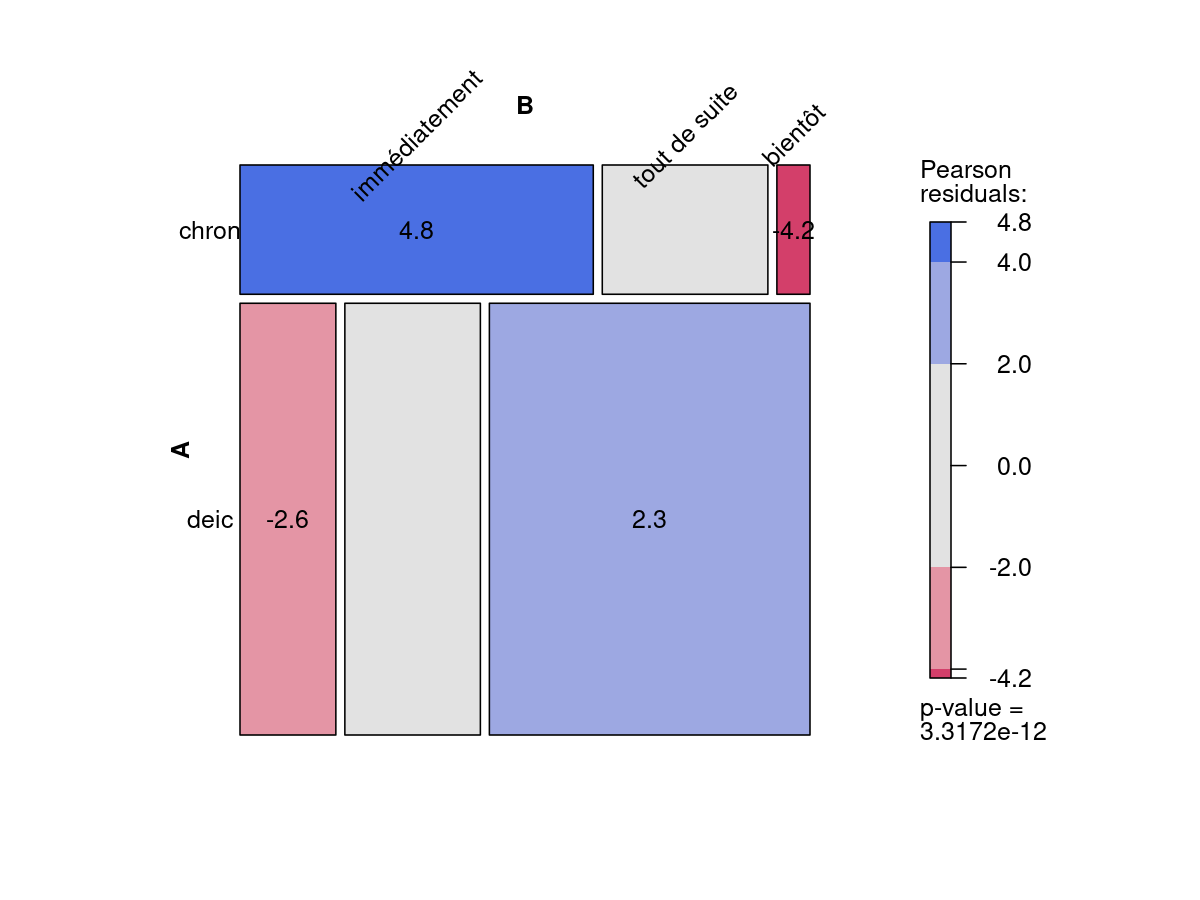
\includegraphics[width=0.9\linewidth]{figures/mosaic-fr-ref-ip.png}
  \cprotect\caption{Contingency table (top) and mosaic plot (bottom)
    representing the frequencies as well as degrees of over- or
    underrepresentation for three French \pradv-adverbials relative to
    the variable \textsc{reference point} (\textit{chron}:
    chronological, \textit{deic}: deictic). The plot was created with
    the package \verb+vcd+ for \verb+R+ (\citealt{vcd-package});
    cf. the script \verb+01_proportional_visualizations.R+ in the
    Supplementary Materials.}
  \label{fig:mosaicplots1-2}
\end{figure}
%
Figure \ref{fig:mosaicplots1-2} also provides information about levels
of deviation from statistical independence (a homogeneous distribution). The
colour of a rectangle corresponding to a cell $C_{m,n}$ of a
contingency table $C$ reflects the magnitude of the Pearson residuals
$E_{m,n}$ for $C_{m,n}$ (cf. \citealt[Ch. 3]{Agresti2002} for
details). Pearson residuals can be regarded as a standardized measure
of deviation from statistical independence. They are calculated as the
difference between the observed and expected frequency, divided by the
square root of the expected frequency (see
Sect. \ref{sec:PearsonResds} in the Appendix for some
explanations). Pearson residuals approximately follow a standard
normal distribution (but see below for a caveat), which means that we
can estimate the probability of a cell count, given the assumption of
statistical independence (homogeneity): $\approx 68\%$ of the data are
located within one standard deviation of the distribution, and
$\approx 95\%$ are located within two standard distributions. As we
are typically interested in results beyond the 95\% threshold
($\alpha=0.05$, for an undirected hypothesis), the thresholds $2$
(for overrepresentation) and $-2$ for underrepresentation are
particularly relevant.

As the legend to the right of the plot shows, the colours indicate the
following magnitudes: light blue: $4 > E_{m,n} > 2$, dark blue: $E_{m,n}>4$,
light red: $-4 < E_{m,n} < -2$, dark red: $E_{m,n}<-4$. In cells with a
significant over- or underrepresentation the Pearson residuals are
moreover specified in the relevant rectangle.
The plot suggests that \textit{immédiatement} tends to co-occur
with chronological reference points, while \textit{bientôt} is
attracted by deictic reference points. \textit{Tout de suite} does not
seem to show a particular association with either type of reference
point.

An important point to note is that Pearson residuals do not exactly
follow a standard normal distribution and ``[provide] conservative
indications of cells having lack of fit'' \citep[81]{Agresti2002}.
Alternatively, an ``adjusted'' residual, which ``results from dividing
it by its standard error'', can be used (\citealt[81]{Agresti2002}). In
the context of mosaic plots, \citet[7]{Friendly1994b} notes that ``the
adjusted residuals are always larger in magnitude than the unadjusted
values'', and ``adjusted residuals have the property that their
standard errors are equal, so their values are more comparable over
cells in the contingency table''. He also holds that ``experience
shows that they provide \textit{better visual display of the patterns
  of association} than do ordinary Pearson \ldots %or LR [linear regression]
residuals'' (emphasis original).

\begin{figure}[t]
  \centering
  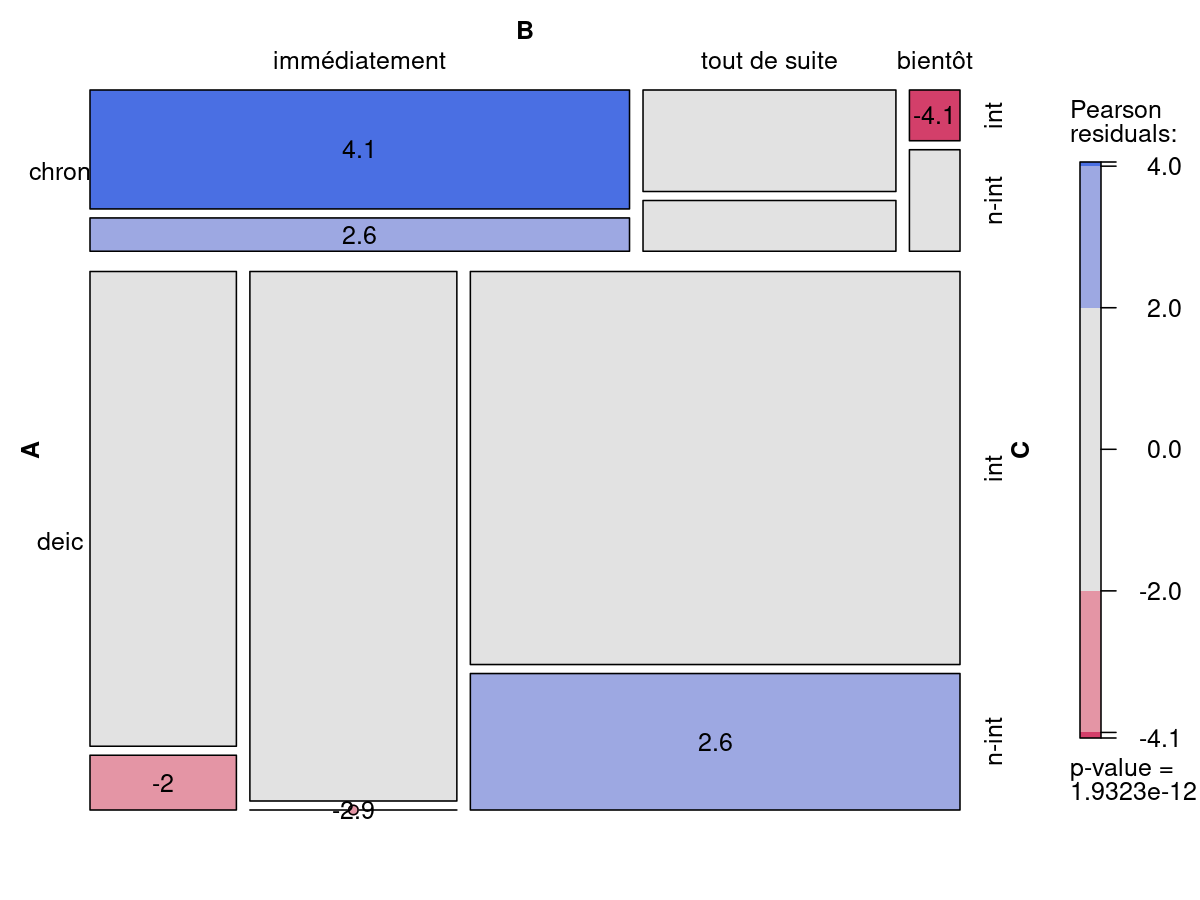
\includegraphics[width=0.9\linewidth]{figures/mosaic-fr-ref-ip-int.png}
  \cprotect\caption{Mosaic plot representing the frequencies as well
    as degrees of over- or underrepresentation for three French
    \pradv-adverbials relative to the variables \textsc{reference
      point} (\textit{chron}: chronological, \textit{deic}: deictic)
    and \textsc{Intentionality} (\textit{int}: intentional,
    \textit{n-int}: non-intentional). The plot was created with the
    package \verb+vcd+ for \verb+R+ (\citealt{vcd-package}); cf. the
    script \verb+01_proportional_visualizations.R+ in the
    Supplementary Materials.}
  \label{fig:2D}
\end{figure}


As we do not focus on inferential statistics in this contribution, we
will not go into any further details at this point (but see
Sect. \ref{sec:PearsonResds} in the Appendix for some
comments). Readers and users should be aware of the ``meaning'' of the
colours in a mosaic plot, however, and take it into account in their
interpretation of the data.
In the following, we will continue to use unadjusted Pearson residuals for the
sake of simplicity, because they also play an important role in
ordination (where they are mostly called `standardized
residuals', see Sect. \ref{sec:Ordination}).

So far we have only crossed two variables. Figure \ref{fig:2D} shows a
mosaic plot where three variables have been crossed: (French)
\textsc{\pradv}, \textsc{Reference Point} and
\textsc{Intentionality}. In this case the (graphically) two-dimensional
representation provided by a mosaic plot has its limitations, and the
diagram effectively shows two plots, one at the top, where
\textsc{Intentionality} is crossed with \textsc{\pradv} for
chronological reference points, and one at the bottom, where this
combination is shown for deictic reference
points. % The information about the residuals
% represented by the colours is based on numbers from the entire
% distribution though.
We can see that three combinations have Pearson residuals higher than $2$:
\{chronological, intentional, \textit{immédiatement}\},
\{chronological, non-intentional, \textit{immédiatement}\},
and \{deictic, non-intentional, \textit{bientôt}\}. \{Deictic,
non-intentional, \textit{immédiatement}\} and \{deictic,
non-intentional, \textit{tout de suite}\} and \{chronological,
intentional, \textit{bientôt}\} have residuals lower than $-2$.

An alternative way of visualizing three-dimensional distributions is
shown in Figure \ref{fig:3D}, in what we call a Feature-Combination
Frequency Grid (FCFG) (see \citealt{Gast2017Even}).  Each node in the
grid corresponds to one feature combination, and the size of a sphere
represents the observed or expected frequency of the relevant feature
combination. The colours of the spheres reflect Pearson
residuals, as in mosaic plots.

\begin{figure}[t]
  \centering
  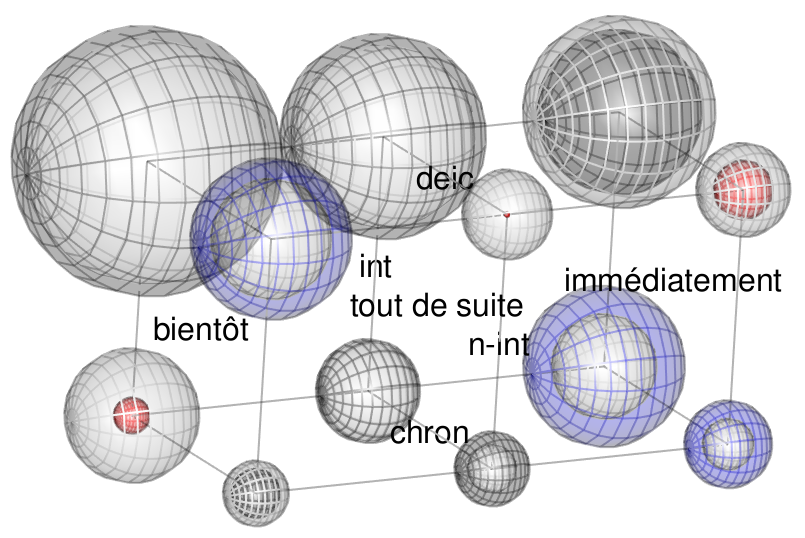
\includegraphics[width=0.5\linewidth]{figures/FCF-grid-ImPost.png}
  \cprotect\caption{Feature-Combination Frequency Grid (FCFG)
    representing the frequencies as well as degrees of over-
    or underrepresentation for three French \pradv s relative
    to the variables \textsc{Illocutionary force} and
    \textsc{Intentionality} (see Fig. \ref{fig:2D} for the
    levels). The visualization was created using the package
    \verb+rgl+ for R; cf. the script
    \verb+01_proportional_visualizations.R+.}
  \label{fig:3D}
\end{figure}


\subsection{Context-Conditional Correlation Graphs}\label{sec:CCCG}

With Feature-Combination Frequency Grids (FCFGs) we can maximally
visualize data along three dimensions. More dimensions are possible
with `stacked' mosaic plots as shown in Figure
\ref{fig:2D}, but the information becomes increasingly difficult
to process as the number of dimensions increases. In order to represent
pairwise associations of variables in a single plot we can make use of
graphs. We call graphs of the type shown in Figure \ref{fig:CCCG}
Context-Conditional Correlation Graphs (CCCG). The graph illustrates
(significant) imbalances in the distribution of German \pradv s
relative to four variables (\textsc{Intentionality}, \textsc{Agent},
\textsc{Reference point} and \textsc{Illocutionary
  force/Modality}).\footnote{Variables and levels:
  \textsc{Agent}: \textit{Ag$x$Ps}
  indicates that \textsc{Agent} is $x$. person;
  %
  \textsc{Illocutionary force/modality}: 
  \textit{dir.boul}: directive/bouletic,
  \textit{n.illoc}: not indicated,
  \textit{poss}: possibility;
  %
  \textsc{Intentionality}: \textit{int}: intentional predicate,
  \textit{n.int}: non-intentional predicate; \textsc{Reference point}:
  \textit{chron}: chronological, \textit{deic}: deictic;
  \textsc{Modification}: \textit{modf}: adverbial is syntactically
  modified, \textit{n-modf}: adverbial is not syntactically
  modified.\label{FigNote1}} The arcs show, for each pair of variables,
the levels for which there is a significant overrepresentation in a
pairwise cross-tabulation, along with the Pearson residual (following
the underscore). For example, the arc at the very top shows that in a
cross-table $T$ of the variables \textsc{\pradv} and \textsc{Agent},
the Pearson residual for the cell $T_{3rd,bald}\approx 4$. The
location of `Ag3ps\_4' (closer to \textit{bald} than to
\textit{gleich}) indicates that this feature is overrepresented for
\textit{bald}.

\begin{figure}[t]
  \centering 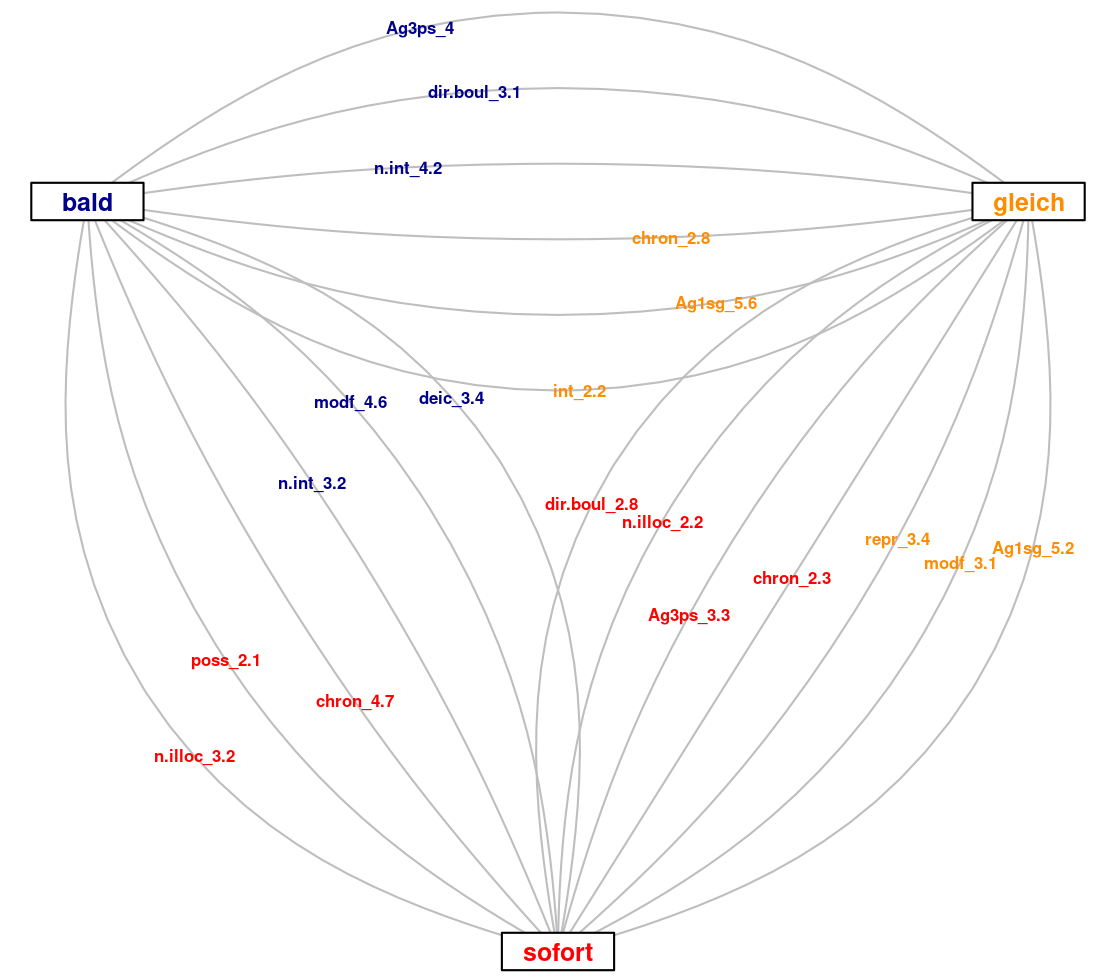
\includegraphics[width=\linewidth]{figures/CCCG-de-ip.png}
  \cprotect\caption{Context-Conditional Correlation Graph; the graph
    visualizes the distribution of German \pradv s relative to four
    variables (\textsc{Intentionality}, \textsc{Agent}, \textsc{Reference point} and
    \textsc{Illocutionary force}; see Note \ref{FigNote1} for the levels). It
    was created with the package \verb+qgraph+ for R
    \citep{qgraph-package}; cf. the script \verb+02_CCCG.R+ in the
    Supplementary Materials.}
  \label{fig:CCCG}
\end{figure}
%
The graph in Figure \ref{fig:CCCG} only shows pairwise associations
and, in a way, summarizes the information distributed over a large
number of $2\times 2$ cross-tables. In order to understand the interplay and
mutual dependencies between the variables in a multivariate data set
like ours, it often makes sense to use ordination techniques, to which
we turn now.

\subsection{Ordination}\label{sec:Ordination}

%The term `ordination' subsumes a number of methods that make use of
%`latent space', i.e., space constituted by latent variables --
%variables that are not directly observable but can be inferred from
%observable (`manifest') variables.
%%
%In the social sciences researchers often
%work with variables that are not measurable but reflected in attitudes
%or behaviour. For example, `sense of belonging' cannot be measured
%directly, but it can be inferred from responses to stimuli such as
%``Spain is my nation'' and ``I feel Spanish''
%\citep{BollenMedrano1998,Bollen2002}.

The term `ordination' subsumes a number of methods that represent multivariate data 
in a low-dimensional space. 
%The resulting dimensions are often interpreted as a `latent space', i.e., a space constituted by latent variables -- variables that are not directly observable but can be inferred from observable (`manifest') variables.
%
%In the social sciences, researchers often work with variables that are not directly measurable but are reflected in attitudes or behaviour.
%For example, a `sense of belonging' cannot be measured directly, but it can be inferred from responses to stimuli such as ``Spain is my nation'' and ``I feel Spanish'' \citep{BollenMedrano1998,Bollen2002}.
%
In this section we discuss two types of ordination techniques that are
useful for the analysis of categorical data, i.e., (simple symmetric)
Correspondence Analysis (Sects. \ref{sec:CA}) and Multiple Correspondence
Analysis (Sect. \ref{sec:MCA}).

\subsubsection{Simple symmetric Correspondence Analysis}\label{sec:CA}

Correspondence Analysis (CA) is probably the most basic type of
ordination (see \citealt{Greenacre2016} for a comprehensive overview
of the ordination techniques discussed in this section). It is based
on the idea that contingency tables can be interpreted as coordinate
systems. Consider the left-hand side of Table \ref{tab:PropTable}. The
table shows rowwise relative frequencies of the German adverbials
\textit{gleich}, \textit{sofort} and \textit{unverzüglich} as
translations of the French \ipadv s \textit{immédiatement} or
\textit{tout de suite} (so essentially it shows the distribution of
German \ipadv s in translations from French).  Each row corresponds to
a `row profile', with the percentages adding up to 1. The columns
represent three levels of the variable \textsc{Illocutionary
  force/modality}, i.e., `comm[issive]' (promises),
`dir[ective]/boul[etic]' (utterances with directive illocutionary
force or bouletic modality, where the speaker expresses a desire,
often amounting to an indirect directive), and `repr[esentative]'
(descriptions of the world).

Without providing any information about significant deviations from
the independence model the row profiles illustrate associations
between levels. For example, the table suggests that \textit{gleich}
is associated with representative illocutionary force, as 72\% of its
cases occur with that level, while for the other adverbials this
column only shows 53\% (\textit{sofort}) and 22\%
(\textit{unverzüglich}).


\begin{table}[b]
  \centering
  \begin{tabular}[h]{l|lll|lll}
    & \multicolumn{3}{l|}{row profiles} & \multicolumn{3}{l}{standardized residuals}\\ \cline{2-7}
    & comm  & dir/boul      &  repr & comm  & dir/boul      &  repr \\\hline
    \textit{gleich}       & 0.16  & 0.12          & 0.72 & 0.11  & -0.23  & 0.13\\
    \textit{sofort}       & 0.06  & 0.41          & 0.53 & -0.1 &  0.09  & -0.03\\
    \textit{unverzüglich} & 0.11  & 0.67          & 0.22 & 0.01  & 0.21   & -0.17 \\\hline
  \end{tabular}
  \caption{Table with row profiles (left) and standardized residuals
    (right) for German \ipadv s in translations from French, relative
    to the variable \textsc{Illocutionary force}}
  \label{tab:PropTable}
\end{table}

We can regard the columns of the left-hand side of Table
\ref{tab:PropTable} as constituting a coordinate system within which
we can locate the three adverbials of interest. This is illustrated in
Figure \ref{fig:Ordination1}. The three axes originating at
$(0\; 0\; 0)$ (the origin) represent the three columns of the left-hand side
of Table \ref{tab:PropTable} and constitute a three-dimensional
coordinate system. The adverbial \textit{unverzüglich}, for instance, is located
at the coordinate $(0.11\; 0.67\; 0.22)$, corresponding to the third
row profile in Table \ref{tab:PropTable} (cf. the orthogonal lines
emanating from the relevant point). The plot also shows the centroid
of the three row points (see Sect. \ref{sec:AppOrdination} in the
Appendix on how the centroid is calculated).

\begin{figure}[t]
  \centering
  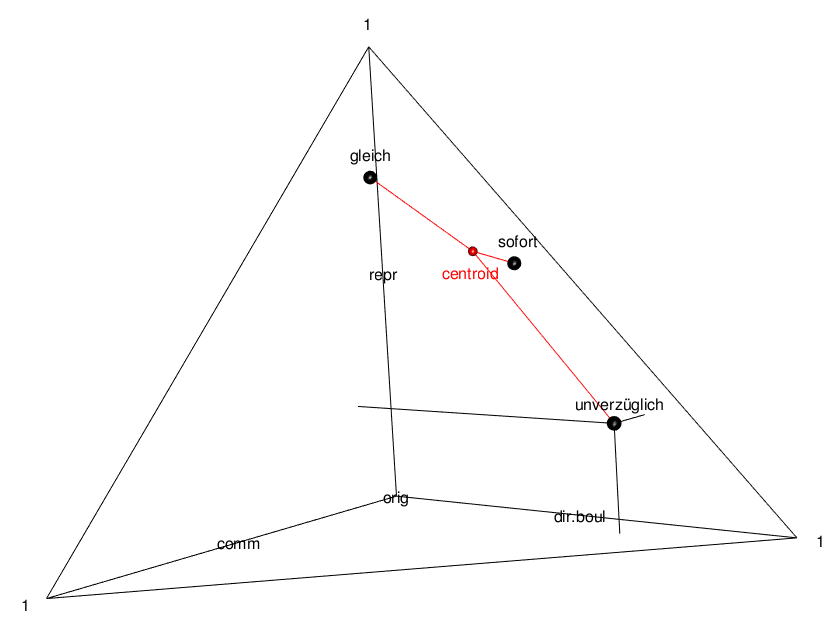
\includegraphics[width=0.75\linewidth]{figures/coord-system-1.png}
  \cprotect\caption{Visualizing Table \ref{tab:PropTable}, with the columns
    constituting a coordinate system for the rows. The plot was
    generated with the package \verb+rgl+ for \verb+R+
    (\citealt{rgl-package}).}
  \label{fig:Ordination1}
\end{figure}

The type of visualization shown in Figure \ref{fig:Ordination1}
constitutes the basis for a lower-dimensional visualization using
CA, which fits a new coordinate system to
the data, in such a way that the largest amount of `inertia'
is captured on a low number of (so-called `principal') axes --
ideally two, as two axes can be easily visualized.
%
Inertia is a measure of spread for count data around the independence
model, corresponding to variance, which is a measure of spread around
the mean value for continuous data.
%
Inertia thus measures the degree to which a contingency table deviates from
statistical independence.
%
The term is inspired by the `moment of inertia' in mechanics, which
quantifies the distribution of mass around an axis of rotation.

CA proceeds as follows:
%
first, the original contingency table (see Table \ref{tab:contingency}
on p. \pageref{tab:contingency}) is converted into a percentage table,
and then into a table of standardized residuals through division by
the square root of the expected percentage (see the right-hand side of
Table \ref{tab:PropTable}; cf. also Sect. \ref{sec:SVD}).
%
As mentioned in Sect. \ref{sec:PropGeom}, Pearson residuals
indicate deviation from independence. The resulting matrix thus
indicates to what extent a cell deviates from the independence model
(assuming a homogeneous distribution).
%
The centroid of the rows constituting this matrix is the origin of a
three-dimensional coordinate system, which is rescaled along the three
axes as a result of the standardization (division by the square root
of the expected frequency). 
The standardized residuals from Table \ref{tab:PropTable} are
visualized in Figure \ref{fig:Ordination3}.

\begin{figure}[t]
  \centering
  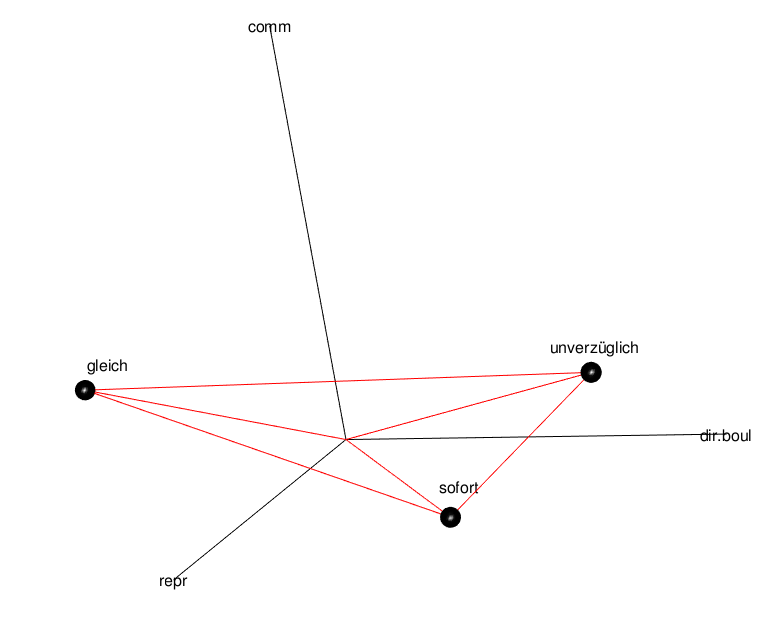
\includegraphics[width=0.75\linewidth]{figures/Ordination3b.png}
  \cprotect\caption{Visualizing the standardized residuals as shown on
    the right-hand side of Table \ref{tab:PropTable}.  The plot was
    generated with the package \verb+rgl+ for \verb+R+
    (\citealt{rgl-package}).}
  \label{fig:Ordination3}
\end{figure}

In a second step, the matrix of standardized residuals is subject to
an operation called `singular value decomposition' (SVD).  The
mathematical procedure of SVD is outlined in
Sect. \ref{sec:AppOrdination} in the Appendix (based on
\citealt{Greenacre2016}). In the main text we will focus on the
results.

SVD fits a new coordinate system to the data, in such a way that the first
(`principal') axis captures most of the inertia, the second axis,
which is orthogonal to the first, captures most of the remaining
inertia, and so on until all data points can be precisely located in
the newly created system.
%
In the case of the data visualized in Figure \ref{fig:Ordination3}, we
can find a coordinate system with only two dimensions that preserves
all the information contained in the table of standardized residuals,
because three points are always located on a (two-dimensional) plane.
If a table has been centered, as in the case
of Pearson residuals, this plane moreover contains the origin
(cf. the triangle in Figure \ref{fig:Ordination3}).

The principal axes determined with SVD %Singular Value Decomposition
constitute the axes of a new coordinate system in which we can locate
both the data points corresponding to the rows of the table of
standardized residuals -- in our case, the \ipadv s \textit{gleich},
\textit{sofort} and \textit{unverzüglich} -- and the original axes
corresponding to the levels of the variable \textsc{Illocutionary
  Force} (`comm', `dir.boul', `repr'). A CA created with the package
\verb+ca+ for \verb+R+ \citep{ca-package} is visualized in Figure
\ref{fig:Ordination2}.\footnote{In Python, the module \verb+prince+
  can be used for CA.}

\begin{figure}[t]
  \centering
  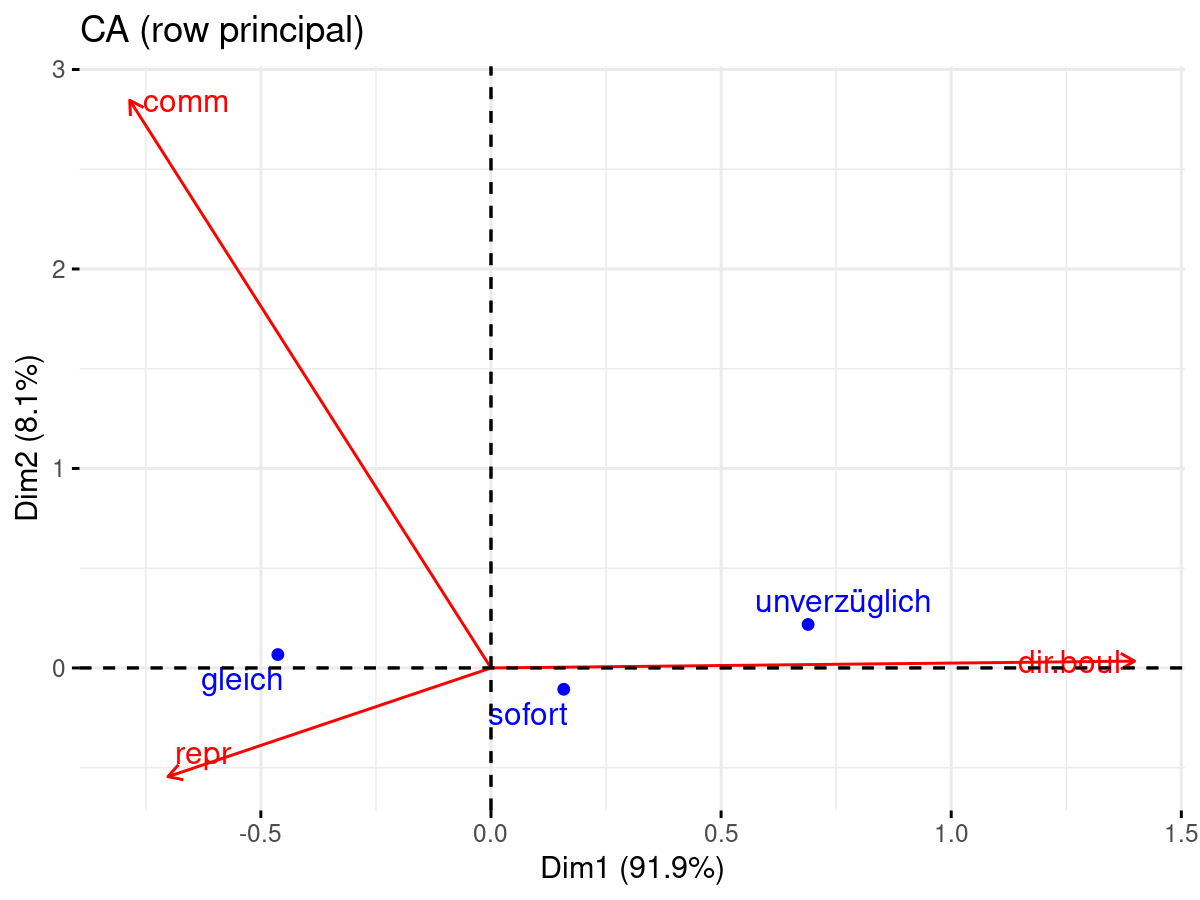
\includegraphics[width=0.75\linewidth]{figures/CA-de-illoc.png}
  \cprotect\caption{Correspondence Analysis for the data in Table
    \ref{tab:PropTable}. The CA was created with the package
    \verb+ca+ for \verb+R+ \citep{ca-package}. For the
    visualization we used the package \verb+factoextra+
    \citep{factoextra-package}. The plot shows a `row analysis', with
    row points in principal coordinates and column vectors in standard
    coordinates.}
  \label{fig:Ordination2}
\end{figure}
%

Along with the two-dimensional representation of the standardized
residuals Figure \ref{fig:Ordination2} shows percentages on both
axes. These percentages indicate how much inertia the
relevant axis covers.
%
Inertia has a direct connection to the Chi-squared test: it is
identical to the Chi-squared statistic, divided by the number of
observations; it is also the square root of the $\phi$-coefficient, a
correlation measure for contingency tables; and it relates directly to
the Chi-squared distances of the row coordinates to the origin. The
Chi-squared distance is defined as the square root of the sum of the
squared differences between the observed values and the expected
values, divided by the expected values. It is a measure of deviation
from independence. 
The inertia of the table is the sum of the Chi-squared distances squared, and
weighted by the row masses.

Consider Figure \ref{fig:Inertia} for
illustration. The left-hand side shows the squared distances of the
three coordinates representing the \ipadv s to the origin,
corresponding to the inertia (without scaling by the row masses). The
right plot shows squares based on the lines that run parallel to the
x-axis (the first principal axis) from the three \ipadv s (also unweighted
by the row masses). The area covered by the squares in the right plot
amounts to $91.9\%$ of the area covered by the total inertia as shown
in the left plot. This is what the percentage on the x-axis in Figure
\ref{fig:Ordination2} indicates.

\begin{figure}[t]
  \centering
  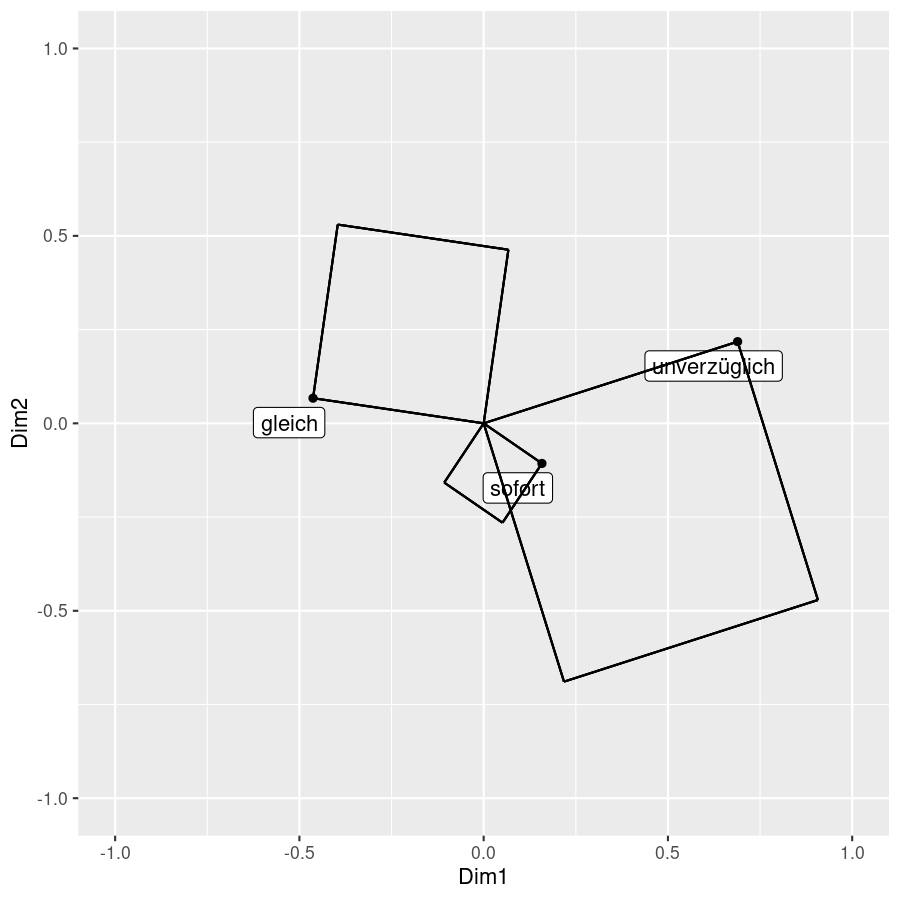
\includegraphics[width=0.45\linewidth]{figures/skewed-rects.png}
  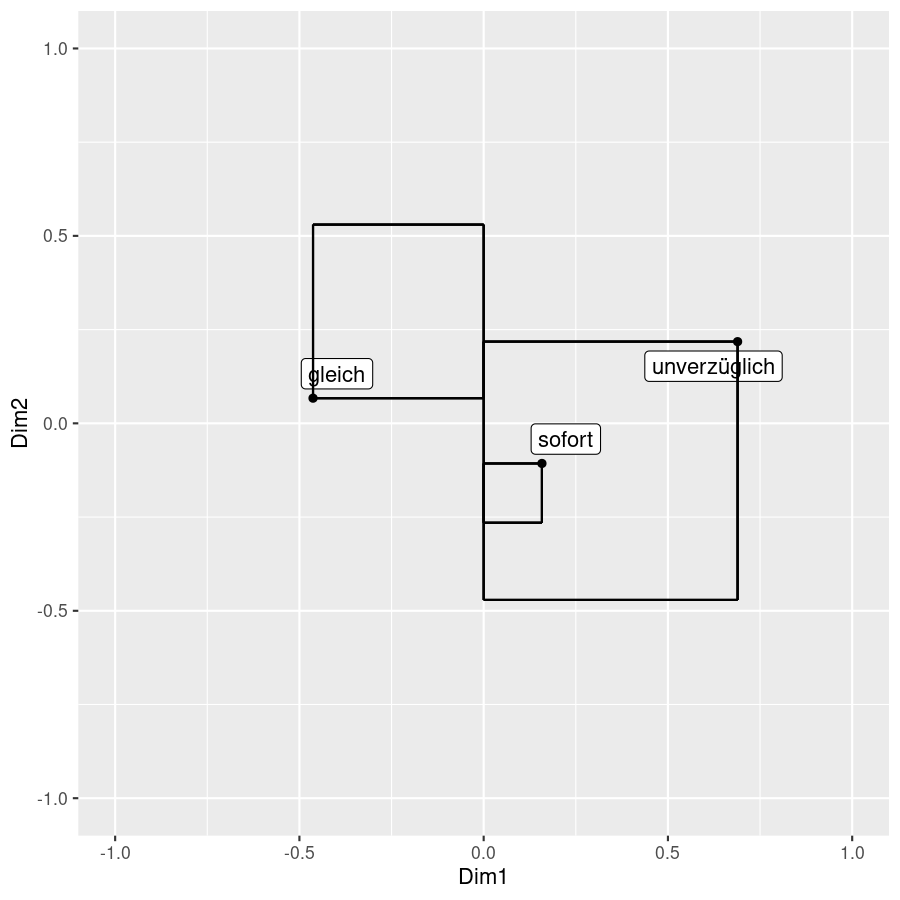
\includegraphics[width=0.45\linewidth]{figures/straight-rects.png}
  \cprotect\caption{Squared Chi-squared distances (left) and squared
    Dimension 1 coordinates (right). The plot was generated with the
    packages \verb+ggplot2+ and \verb+ggrepel+ for \verb+R+
    \citep{ggplot2-package,ggrepel-package}.}
  \label{fig:Inertia}
\end{figure}

The inertia not only gives us information about the
degree of truthfulness of the dimensionality-reduced representation
relative to the original, higher-di\-mension\-al one, it also tells us how
`important' specific axes are. When looking at Figure
\ref{fig:Ordination2} one might be led to believe that the two axes
explain a similar amount of inertia; but Axis 1 alone explains $\approx 92\%$ of
it. 
Note that all adverbials as well as the two
levels of \textsc{Illocutionary force} (`repr', `dir/boul') are very close to
the $x$-axis -- with low values on the $y$-axis --, implying that the
$y$-axis explains a low amount of their row inertia.

So far we have focused on the position of the points representing the
rows (\ipadv s) in what is called a ``row analysis'' of CA. Remember
that our starting point was the location of \ipadv s relative to distributional
variables, which constitute a coordinate system within which we can locate the
latter. In principle, CA is symmetrical and we could just as well
locate columns relative to rows. In fact, there are many ways of
visualizing CAs, implemented, for instance, in the
\verb+fviz_ca_biplot+ function of the \verb+factoextra+ package
\citep{factoextra-package}, or the \verb+plot.ca+ function of the
\verb+ca+ package for \verb+R+ \citep{ca-package}.  In a row analysis
the rows (\ipadv s) are represented in so-called `principal
coordinates', which preserve Chi-squared distances between the
observations. The columns, represented as vectors in Figure
\ref{fig:Ordination2}, are displayed in `standard coordinates', which are
so-called because they have a mean value of 0 and a variance of 1
\citep[62]{Greenacre2016}.

\hyphenation{gleich}

In this display the relationship between an \ipadv\ (row) and a
variable (column) is not represented by the distances between row and
column vectors; it (ideally) corresponds to the inner products of
these vectors (``ideally'' bacause information may be lost as a result
of the dimensionality reduction). This means that the degree of
association between a row and a column is a function of the degree to
which the two vectors point in the same direction. If all of the
information has been preserved, we can reconstruct the values
of the original table from the map shown in Figure
\ref{fig:Ordination2}. For example, the standardized residual for the
combination \textit{gleich}/`repr' is the inner product of the two
vectors for \textit{gleich} (scaled by the square root of its row
mass) and the vector pointing at `repr' (scaled by the square root of
the average profile; see \citealt{Greenacre2016} for more information
and Sect. \ref{sec:AppOrdination} in the Appendix for the calculation of this
example).

While not everybody may be interested in the mathematical details, it
is important to be aware of the specific type of map that is used for
visualization. The `row principal' representation chosen in Figure
\ref{fig:Ordination2} is rather transparent, but often has the
disadvantage of a visual imbalance between the row points, which are
closer to the centre, and the column points, which are spread out
more. Users should be aware, however, that a representation that
condenses the data -- while visually being more pleasing --
potentially does not have the inner product interpretation of an
asymmetric row principal plot, where the rows are represented in
principal coordinates, and the columns in standard coordinates (see
\citealt[Ch. 13]{Greenacre2016} for discussion).

Representations like the one in Figure \ref{fig:Ordination2} give us
an idea of the relationship between the levels of two
variables. However, with a multivariate data set like ours, we need to
be able to represent relationships between more than one variable. A
very simple way of visualizing more than one variable is provided by a
`stacked' CA \citep[Ch. 17]{Greenacre2016}. We can simply concatenate
contingency tables (horizontally or vertically) and carry out a CA on
that table. Horizontal concatenation is illustrated for our data in
Table \ref{tab:StackedContingency}, which shows the percentages for
the variable \textsc{Illocutionary force} on the left, and for
\textsc{Agent} on the right.

\begin{table}[t]
  \centering
  \begin{tabular}[h]{l|lll|llll}
             &  comm  &  dir.boul &  repr &  1pl  &  1sg  &  2ps  &  3ps\\\hline
\textit{gleich}       &  0.08  &  0.06     &  0.36 &  0.06 &  0.22 &  0.06 &  0.16\\
\textit{sofort}       &  0.03  &  0.21     &  0.26 &  0.07 &  0.01 &  0.06 &  0.35\\
\textit{unverzüglich} &  0.06  &  0.33     &  0.11 &  0.06 &  0.00 &  0.00 & 0.44\\
  \end{tabular}
  \caption{Stacked contingency table for German \ipadv s (in
    translations from French) and the explanatory variables
    \textsc{Illocutionary force} and \textsc{Agent}}
  \label{tab:StackedContingency}
\end{table}
%
Given that the number of observations per variable is invariant, the
Chi-squared distances between the levels of each variable are preserved
in this type of stacked CA. The positions of the various levels
relative to each other are thus not affected by the stacking
(cf. Figure \ref{fig:Ordination5}). However, it is clear that some
information is lost in a stacked CA, as we do not get any information
about the relationship between the levels of the explanatory variables
(here, \textsc{Illocutionary force} and \textsc{Agent}). Table
\ref{tab:StackedContingency} suggests that a certain number of
ocurrences of \textit{gleich} have commissive illocutionary force, and
another set of observations has a first person agent. The table does
not tell us how many of the commissive observations have first person
agents. In other words, the distributional variables are treated as
being independent. While this is a clear drawback of the stacked CA,
the method can be useful in order to determine the degree of
independence of predictor variables. In particular, it can be
instructive to compare a stacked CA to a Multiple Correspondence
Analysis, to which we turn next.

\begin{figure}[b]
  \centering
  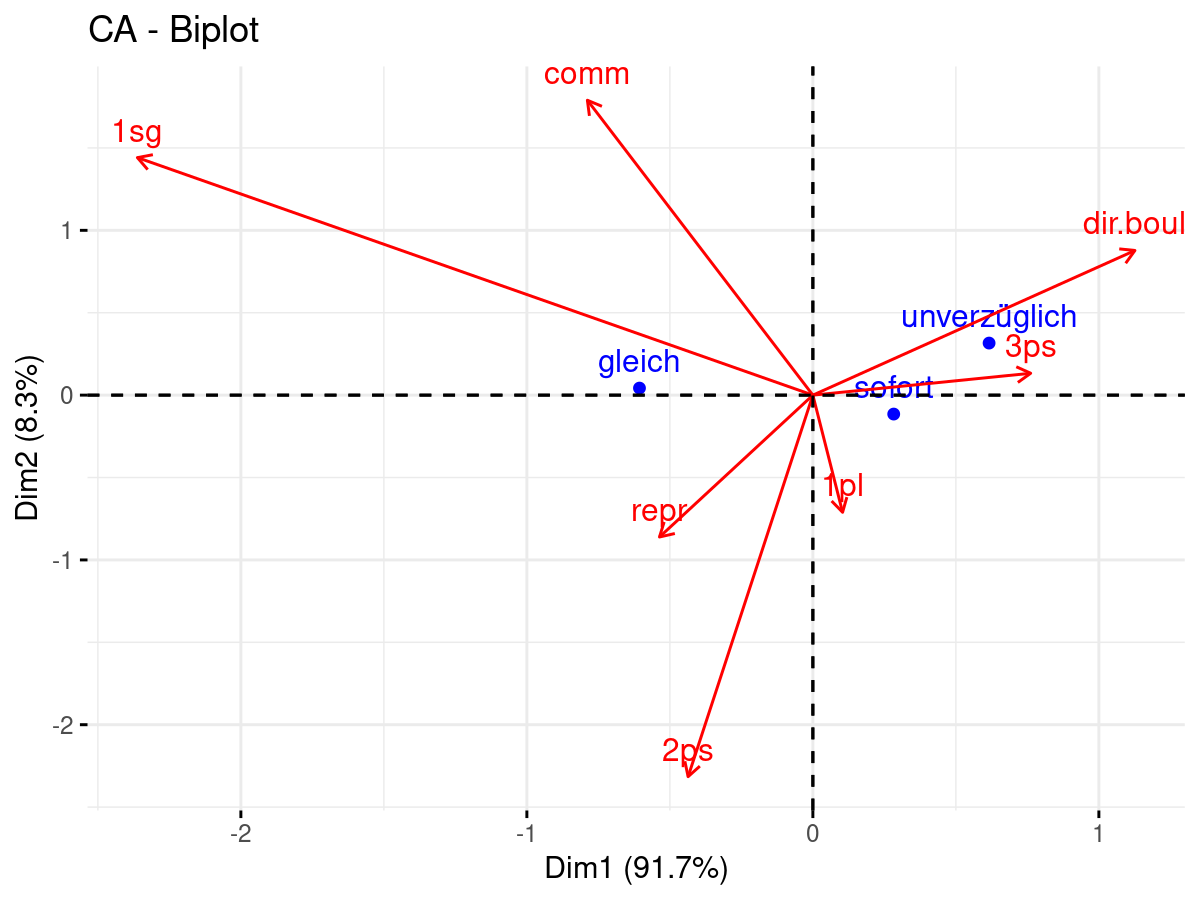
\includegraphics[width=0.67\linewidth]{figures/CA-de-stacked.png}
  \cprotect\caption{Stacked Correspondence Analysis showing the
    location of three German \pradv s in a coordinate system derived from their associations with
    the variables \textsc{Illocutionary force} and \textsc{Agent}. The
    CA was fitted with the package \verb+ca+ for \verb+R+
    (\citealt{ca-package}) and the plot was created with the package
    \verb+factoextra+ for \verb+R+ \citep{factoextra-package}.}
  \label{fig:Ordination5}
\end{figure}

\subsubsection{Multiple Correspondence Analysis}\label{sec:MCA}

From a mathematical point of view, Multiple Correspondence Analysis
(MCA) functions very much like (simple) CA. However, it is based on a
representation of the data that takes the relationships between all
(explanatory as well as response) variables into account. There are
two (near equivalent) ways of accomplishing this: (i) carrying out a CA on
the indicator matrix of a data set, or (ii) using the Burt table
instead.

An indicator matrix is a binary matrix that indicates whether
or not an observation exhibits a given property.
%
Consider Table \ref{tab:RandomDF}, which shows a random fragment of
our data frame (German translations of French \ipadv s). Each row corresponds to
one example, and the columns specify the illocutionary force, the Agent, and
the German adverbial.

\begin{table}[H]
  % \centering
  \small
  \begin{tabular}[h]{llll}
  ID  &    \textsc{Illoc}    & \textsc{Agent}    & German \textsc{\ipadv}\\\hline
  214 &   repr      &    1sg   &    \textit{sofort}\\
  216 &   dir.boul  &    1pl   &    \textit{sofort}\\
  217 &   repr      &    3ps   &    \textit{gleich}\\
  218 &   repr      &    3ps   &    \textit{sofort}\\
  221 &   dir.boul  &    3ps   &    \textit{unverzüglich}\\
  \end{tabular}
  \caption{Random fragment of the data frame}
  \label{tab:RandomDF}
\end{table}
%
The indicator matrix corresponding to Table \ref{tab:RandomDF} is
shown in Table \ref{tab:RandomDFIndicator}.
%
Here, each column corresponds to a level of a variable, not a variable. While
Table \ref{tab:RandomDF} specifies the levels themselves in the cells,
Table \ref{tab:RandomDFIndicator} shows whether (1) or not (0) the observation
in question is an instance of the relevant level.

\begin{table}[H]
  % \centering
  \small
  \begin{tabular}[h]{l|rrr|rrrr|rrr}
    & \multicolumn{3}{c|}{\textsc{Illoc}} & \multicolumn{4}{c|}{\textsc{Agent}} & \multicolumn{3}{c}{\textsc{\ipadv}}\\ 
    &   comm & dir.boul & repr & 1pl & 1sg & 2ps & 3ps & \textit{gleich}& \textit{sofort} & \textit{unvzgl.}\\\hline
214 &     0  & 0        &  1    &   0 & 1           & 0           & 0           & 0           & 1       & 0\\
215 &     0  & 1        &  0    &   1 & 0           & 0           & 0           & 0           & 1       & 0\\
216 &     0  & 0        &  1    &   0 & 0           & 0           & 1           & 1           & 0       & 0\\
217 &     0  & 0        &  1    &   0 & 0           & 0           & 1           & 0           & 1       & 0\\
218 &     0  & 1        &  0    &   0 & 0           & 0           & 1           & 0           & 0       & 1\\    
  \end{tabular}
  \caption{Indicator matrix corresponding to Table \ref{tab:RandomDF}}
  \label{tab:RandomDFIndicator}
\end{table}

A Burt matrix is a cross-tabulation of the frequencies of all levels of
all variables with all other levels of all other variables. Table
\ref{tab:BurtMat} shows a fragment of our data in the form of a Burt
matrix. Burt matrices and indicator matrices are systematically
related insofar as the Burt matrix is the inner product of the
transpose of the indicator matrix with itself ($B=I^\mathsf{T}I$, for
an indicator matrix $I$).

While MCA is ``mathematically'' quite similar to CA, 
from the point of view of interpretation the two techniques are quite
different. In CA, the rows correspond to categories of interest and the
columns to the levels of a variable. In MCA, the rows correspond to
individual observations (in the indicator matrix) and the columns
correspond to variables that the individuals do (not) exhibit. Unlike
CA, MCA thus provides information about individual
observations. Moreover, in MCA \textit{all} (levels of) variables are
related to each other via Chi-squared distances.


\begin{table}[t]
  \centering
  \begin{tabular}[h]{l|lll|lll}
               & \textit{gleich} & \textit{sofort} & \textit{unverzüglich} & comm & dir.boul &repr\\\hline
\textit{gleich}         & 25            & 0                  & 0                & 4 & 3               & 18\\
\textit{sofort}         & 0           & 34                  & 0                & 2 & 14               & 18\\
\textit{unverzüglich}   & 0            & 0                  & 9                & 1 & 6                & 2\\\hline
comm           & 4            & 2                  & 1                & 7 & 0                & 0\\
dir.boul       & 3           & 14                  & 6                & 0 & 23                & 0\\
repr           & 18           & 18                  & 2                & 0 & 0               & 38\\
  \end{tabular}
  \caption{Burt matrix corresponding to Table \ref{tab:RandomDF}}
  \label{tab:BurtMat}
\end{table}

A downside of MCA is that the underlying data tables -- the indicator
matrix (Table \ref{tab:RandomDFIndicator}) or the Burt matrix (Table
\ref{tab:BurtMat}) -- are highly redundant. The indicator matrix
contains a lot of zeros, which turn into negative values when the
residuals are calculated. The Burt matrix contains a lot of
uninformative material on the diagonal, where levels are crossed with
themselves. Because of the redundancy, both tables inflate the overall
inertia. As a result, MCAs typically appear to explain a low
percentage of inertia on their first principal axes.
%
\citet{Greenacre2016} has proposed a way of `adjusting' the inertia in
MCAs, which is implemented in the package \verb+ca+ for
\verb+R+ \citep{ca-package}. 

Figure \ref{fig:Ordination6} shows an MCA for German translations of
French \ipadv s, with three variables: \textsc{\ipadv},
\textsc{Illocutionary force} and \textsc{Agent}.\footnote{We used the
  package \verb+FactoMineR+ for \verb+R+
  \citep{FactoMineR-package}. In Python, the module \verb+prince+ can
  be used for MCAs.} Without adjustment, the percentage of inertia
captured by the first two principal axes is 26.3\% (Axis 1) and 19.2\%
(Axis 2). It is much higher when computed with Greenacre's (2016)
adjustment (72.7\% [Axis 1] and 11.0\% [Axis 2]).

\begin{figure}[t]
  \centering
  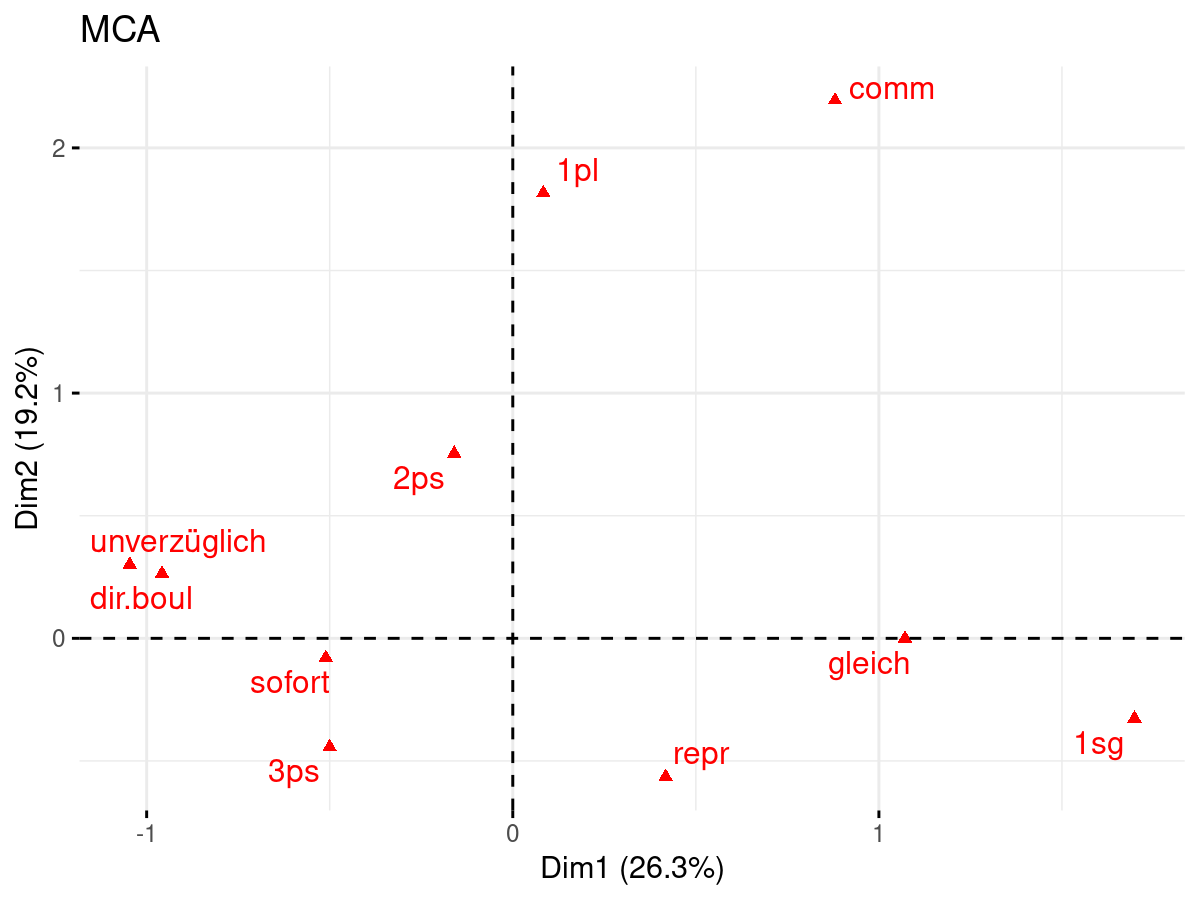
\includegraphics[width=0.75\linewidth]{figures/MCA-de-trl.png}
  \cprotect\caption{Multiple Correspondence Analysis for the variables
    \textsc{Illocutionary force}, \textsc{Agent} and \textsc{\ipadv}
    (German translations of French \ipadv s). The MCA was fitted with
    the package \verb+FactoMineR+ for \verb+R+
    \citep{FactoMineR-package}, the plot was generated using the
    package \verb+factoextra+ \citep{factoextra-package}.}
  \label{fig:Ordination6}
\end{figure}

An MCA creates a new coordinate system that is structured by all variables
relative to all other variables. It creates a mapping from frequency
distributions to positions in this system. We can therefore also locate
variables (and observations) in MCA-coordinates without them being used
to create those coordinates. In MCA speech, this means that we use
`supplementary' (or `passive') variables. In a data set like ours it
often makes sense to treat the target variable -- in our case,
expressions of immediate or proximal posteriority -- as a
supplementary variable. The idea is that the MCA-coordinates are
defined by explanatory variables only, and that the adverbials in
question can be located in terms of these coordinates. This is shown in
Figure \ref{fig:Ordination7} for the same data that was used to
generate the stacked CA in Figure \ref{fig:Ordination5}, and the MCA
without supplementary variables in Figure \ref{fig:Ordination6}.


\begin{figure}[t]
  \centering
  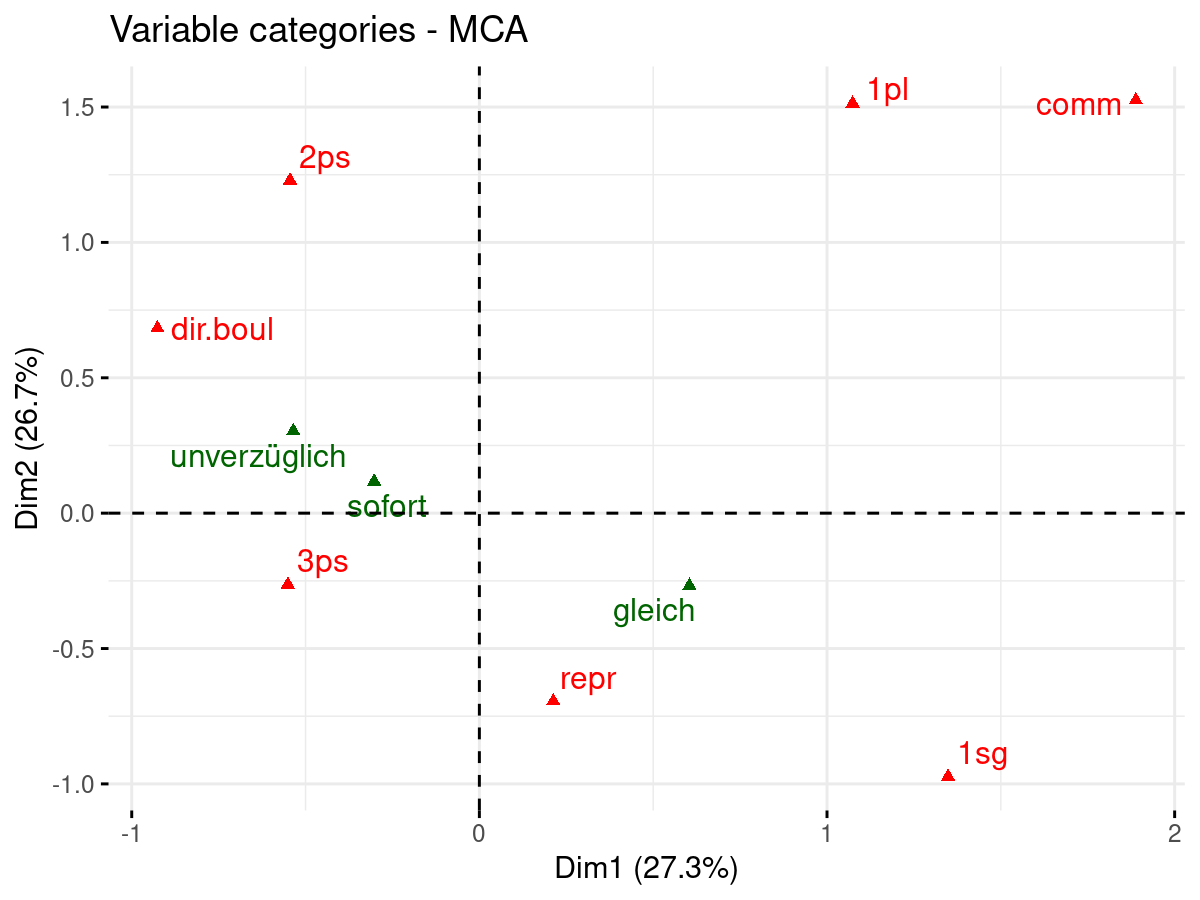
\includegraphics[width=0.75\linewidth]{figures/MCA-supp-de-trl.png}
  \cprotect\caption{MCA for the variables \textsc{Illocutionary force}
    and \textsc{Agent}, with \textsc{\ipadv} as a supplementary
    variable (German translations of French \ipadv s).)  The MCA was
    fitted with the package \verb+FactoMineR+ for \verb+R+
    \citep{FactoMineR-package}, the plot was generated using the package
    \verb+factoextra+ \citep{factoextra-package}.}
  \label{fig:Ordination7}
\end{figure}

\subsection{Comparing CA and MCA}\label{sec:OrdionationComparison} 

The three ordination methods mentioned above provide ways of
displaying different types of interdependencies between variables. A
stacked CA represents the data in a coordinate system derived from the
association between rows and columns, and positions the rows
(adverbials) relative to the columns (distributional variables), or
vice versa (the method is symmetric, although our focus has been on the
row analysis). CA visualizes relations between context variables
and adverbials, but not relations among the context variables
themselves.

An MCA with supplementary variables, in a sense, emphasizes the
opposite perspective: it constructs a space based on the relationships
among the context variables, and then projects the adverbials into this
space. An MCA without supplementary variables represents relationships
among all variables simultaneously, i.e., it does not distinguish
between context variables and adverbials.


The differences between the three types of visualizations can be
illustrated with the relationship between one German adverbial,
\textit{unverzüglich}, and two context variables,
\textsc{Illocutionary force} and \textsc{Agent}. Consider first the
(stacked) CA shown in Figure \ref{fig:Ordination5}. The \ipadv\
\textit{unverzüglich} and the category `2nd person' are located on opposite
ends of the origin, suggesting a negative association. As a matter of
fact, the variables are complementary, in the sense that
\textit{unverzüglich} is never used with the second person in our
sample. In Figures \ref{fig:Ordination6} (MCA without supplementary
variables) and \ref{fig:Ordination7} (MCA with supplementary
variables), the second person is located in the same quadrant as
\textit{unverzüglich}. The reason is that both categories are
distributionally related to directive illocutionary force or bouletic
modality (`dir.boul'), though not to each other. In a way, the MCAs
suggests a deceiving distributional association between
\textit{unverzüglich} and the second person.
%
What this example illustrates is that none of the three methods
considered above -- stacked CA, MCA with or without supplementary
variables -- can, in itself, provide a complete picture of the
data. It is therefore instructive to experiment with different methods
in order to develop a better understanding of the data. This does not
mean, of course, that readers should feel encouraged to cherry pick
those plots that they like best. Remember that the primary focus of this
contribution is to support researchers in understanding their data,
not in applying inferential statistics.

%%% Local Variables:
%%% mode: latex
%%% TeX-master: "main"
%%% End:

\section{Visualizing undirected comparative distributions}\label{sec:ComparativeUndirected}

In order to compare two languages in terms of the way a given
functional domain is structured, a common procedure is to use a
semantic or functional criterion as a third of comparison, and then
determine the way the semantic space in question is mapped to linguistic expressions \citep{Gast2012}. In our case, this means that
we use the functional annotations as a \textit{tertium comparationis},
and we locate the expressions from different languages relative to
these annotations.

In Sect. \ref{sec:LanguageSpecific} we used four methods to visualize
form-function mappings in specific languages: CA -- with and without
stacked tables -- and MCA -- with and without supplementary variables. In this
section we focus on only one of these methods, MCA with
supplementary variables. The advantage of an MCA over a CA (with
stacked tables) is that it allows us a per-item analysis, as each
observation, and not just the variables, are located in low-dimensional space. The advantage of an MCA with supplementary variables is that it
creates a coordinate system that is independent of the specific expressions
used in a language, so we can (comparatively) locate expressions from
different languages in that system. Put differently, the coordinate system is
constituted by the distributional variables, functioning as the
\textit{tertium comparationis}, while the expressions are the  \textit{comparanda}.

An MCA with `IP-adverbial' as a supplementary variable is shown for
original occurrences of \textit{gleich}, \textit{sofort},
\textit{immédiatement} and \textit{tout de suite} in Figure
\ref{fig:MCADeFrSup}, relative to four distributional variables
(\textsc{intentionality}, \textsc{Agent}, \textsc{Illocutionary force}
and \textsc{Reference point}).


\begin{figure}
  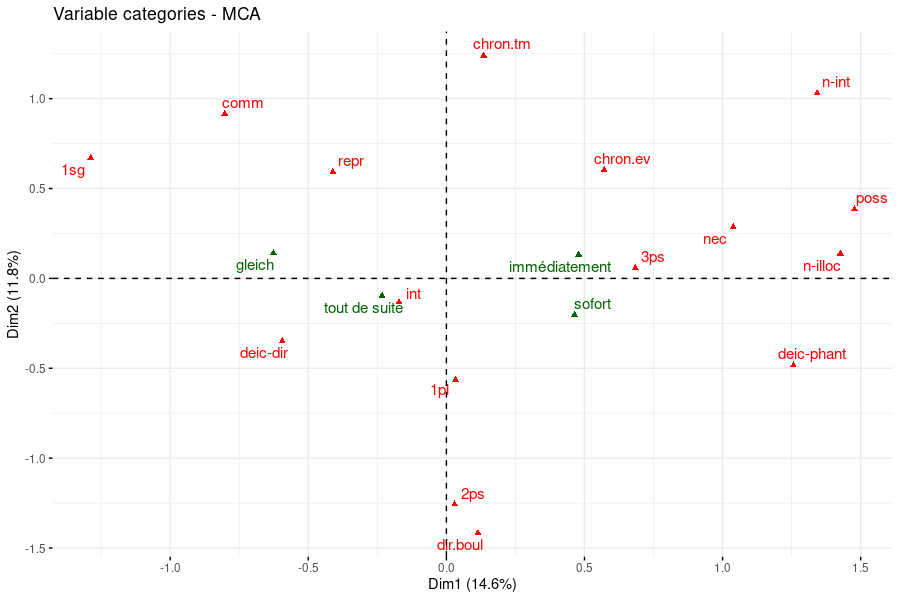
\includegraphics[width=\linewidth]{figures/MCA-sup-de-fr.png}
  \cprotect\caption{MCA with IP-adverbial as supplementary variable
    (German and originals), relative to the variables
    `intentionality', `agent', `illocutionary force' and `reference
    point'. The CA was created with the package \verb+FactoMineR+ for
    \verb+R+ \citep{FactoMineR-package}, for the visualization we used
    the package \verb+factoextra+ \citep{factoextra-package}. The
    adjusted percentages of explained inertia as returned by the
    package \verb+ca+ for \verb+R+ \citep{ca-package} are 48.5\% (Axis
    1) and 15.0\% (Axis 2).}
  \label{fig:MCADeFrSup}
\end{figure}

Though no doubt quite informative, Figure \ref{fig:MCADeFrSup} is
hard to read. A general observation that stands out is that
the four adverbials are located in different quadrants of the
plot. Another relevant observation is that \textit{tout de suite} is
considerably closer to the centre than the other adverbials, which
suggests a less specialized distribution for this adverbial.

One way of simplifying a multivariate distribution as shown in Figure
\ref{fig:MCADeFrSup} is to apply clustering. As an MCA locates every
single observation in the new space that it creates, we can
identify clusters of similar observations. We used PAM (partitioning
around medoids) clustering for this purpose, which identifies clusters
on the basis of distances between observations -- as the name
suggests, around a medoid, i.e., a (representative) observation in the
centre of the cluster. \footnote{We used the package \verb+cluster+
  for \verb+R+, cf. \citet{cluster-package}. We validated the
  clustering solution using the silhouette method (see the package
  documentation for more information).} Clusters with 3 or 6 medoids
were chosen because the average silhouette scores showed visible leaps
at these points (in comparison to solutions with 2 and 5 clusters; see
Figure \ref{fig:Silhouette}, Sect. \ref{sec:AppComparativeUndirected},
in the Appendix). The location of clusters of individual sentences in
the coordinate system defined by the MCA is visualized in Figure
\ref{fig:MCACluster}.
%
The annotations for the medoid observations of the clusters are shown
in Table \ref{tab:Medoids}. The corresponding examples are provided in
\bv{ClusterEx1}--\bv{ClusterEx3}. 

\pagebreak

\begin{table}[H]
  \centering
  \scriptsize
    \begin{tabular}[h]{llllll|llllll}
    ID  & agent &int &mod   &   ref & cl & ID  & agent &int &mod   &   ref & cl \\\hline
    448   &1sg &int     &repr &deic-dir & 1 & 448   &1sg   &int     &repr   &deic-dir  &     1 \\
    16    &3ps &int     &repr &chron.ev & 2 & 41    &3ps   &int     &repr   &deic-dir  &     2 \\
    443   &3ps &int &dir.boul &deic-dir & 3 & 443  & 3ps   &int &dir.boul   &deic-dir  &     3 \\
    &   &&&&&441   &3ps   &int   &  repr &  chron.ev &      4\\
    &   &&&&&455   &3ps   &int &dir.boul &  chron.ev  &     5\\
    &   &&&&&280   &3ps &n-int  &   repr &deic-phant  &     6\\
  \end{tabular}
  \caption{Medoid observations for cluster solutions with 3 (left) and 6 (right) clusters}
  \label{tab:Medoids}
\end{table}

\begin{exe}
  \ex\label{ClusterEx1}
  \begin{xlist}
    \ex Je lui donne bien volontiers tout de suite la parole. (original)
    \ex Ich erteile ihm daher gern sogleich das Wort.
    \ex I am very happy to give you the floor now.
  \end{xlist}
  \ex\label{ClusterEx2}
  \begin{xlist}
    \ex C'est une expérience amère, lorsque l'on fait des propositions
    de réforme, de constater que d'autres les bloquent constamment
    avec des référence à autre chose.
    \ex Ich finde es bitter, wenn
    man Reformvorschläge macht, dass die gleich immer so abgeblockt
    und mit etwas anderem in Bezug gebracht werden. (original)
    \ex It is a bitter experience, when one makes reform proposals, to find
    that others are constantly blocking them with reference to
    something else.
  \end{xlist}
  \ex\label{ClusterEx3}
  \begin{xlist}
    \ex Il faut mettre ce régime sous tutelle internationale et il faut le faire tout de suite!
    \ex Dieses Regime muß unter internationale Aufsicht gestellt werden, und zwar sofort! (original)
    \ex This regime needs to be placed under international supervision, and this should be done straight away! 
  \end{xlist}
\end{exe}
%
In the French and German versions of the medoid of Cluster 1
(cf. \bv{ClusterEx1}) we find \textit{tout de suite} and
\textit{sogleich}, arguably a stylistic variant of
\textit{gleich}. The medoid of Cluster 2 (cf. \bv{ClusterEx2}) also
has \textit{gleich} in German but no expression in French -- a not
uncommon situation. The medoid of Cluster 3 (cf. \bv{ClusterEx3}) has
\textit{sofort} in German and \textit{tout de suite} in French. This
illustrates that the clusters are not actually constituted by German
or French expressions. They represent characteristic utterance types
defined by the distributional variables: (i) a (typically deictic)
declaration of future action by the speaker (Cluster 1); (ii) a
(typically chronological) statement about a third person (Cluster 2);
and (iii) a call for action (Cluster 3).

\begin{figure}[t]
  \centering
  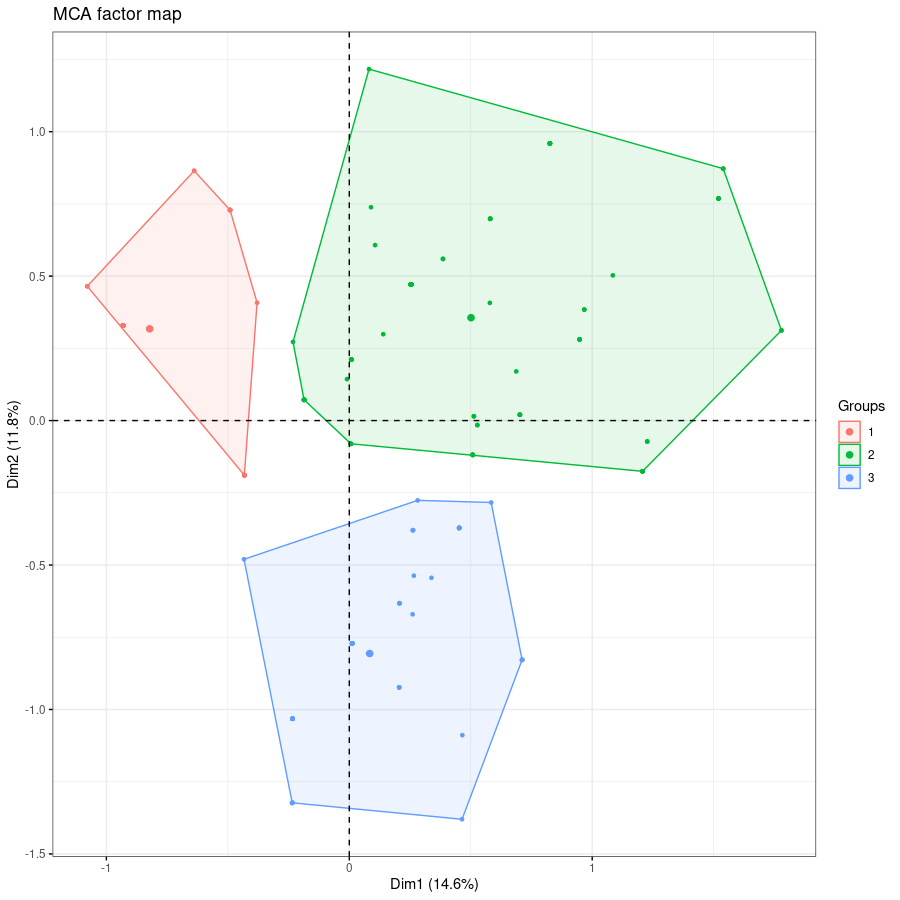
\includegraphics[width=0.45\linewidth]{figures/cluster-low.png}
  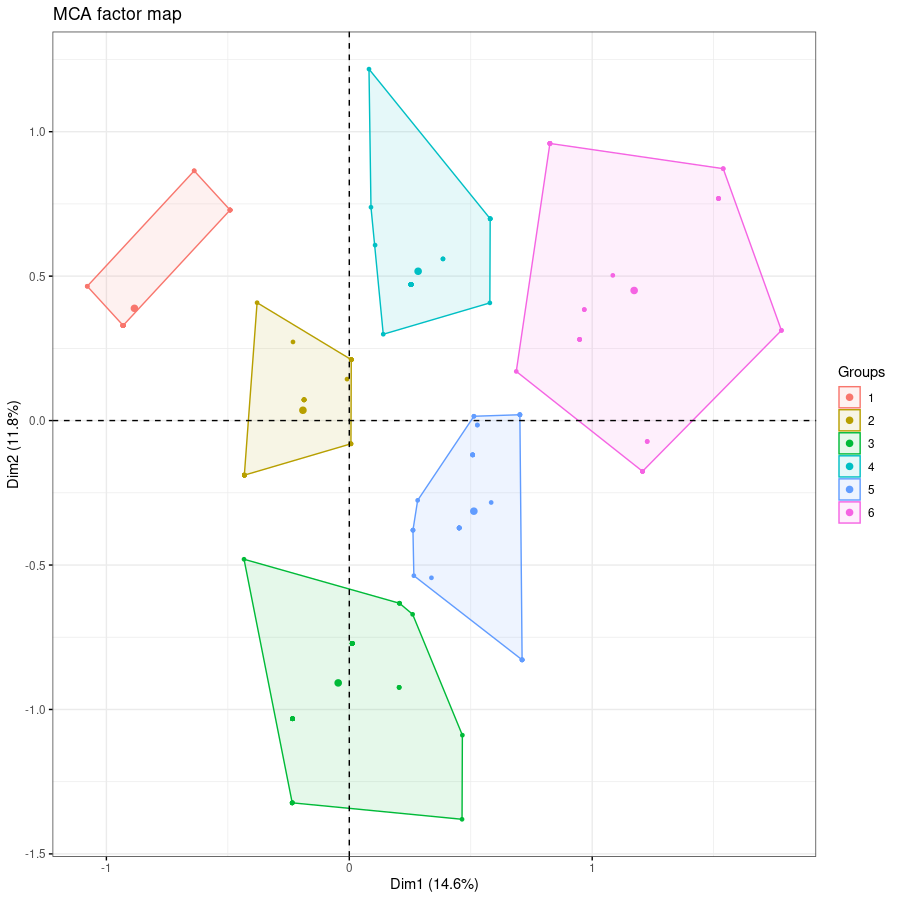
\includegraphics[width=0.45\linewidth]{figures/cluster-high.png}
  \cprotect\caption{Clusters based on MCA-coordinates and
    PAM-clustering with three (left) and six (right)
    clusters, using the package \verb+cluster+ for \verb+R+
    \citep{cluster-package}. The plots were generated with the package
    \verb+factoextra+ for R \citep{factoextra-package}.}
  \label{fig:MCACluster}
\end{figure}
%
In order to understand associations between clusters (major use types)
and \ipadv s we can cross-tabulate the \ipadv s with the clusters of
the two cluster solutions. Relevant mosaic plots are shown in Figure
\ref{fig:MosaicClusters}. Both plots suggest a positive association of
Cluster 1 with \textit{gleich}. The plot with six clusters moreover
shows positive associations between \textit{immédiatement} and Cluster
6, and between \textit{sofort} and Cluster 5. Another important
observation is that \textit{tout de suite} does not show an
association with any of the clusters. This confirms our impression
that it is the most generic/least specialized expression of the \ipadv
s under investigation.

\begin{figure}[b]
  \centering
  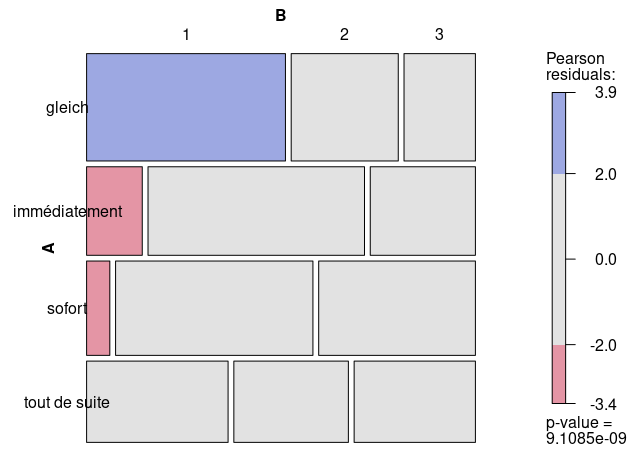
\includegraphics[width=0.45\linewidth]{figures/mosaic-cluster-low.png}
  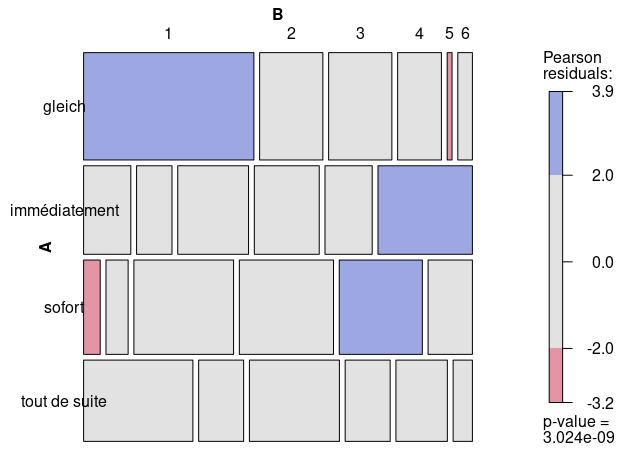
\includegraphics[width=0.45\linewidth]{figures/mosaic-cluster-high.png}
  \cprotect\caption{Mosaic plots for cross-tabulations of German and French
    \ipadv s with clusters, for cluster solutions with three (left) and six (right)
    clusters. The plots were generated with the package \verb+vcd+ for
    \verb+R+ \citep{vcd-package}.}
  \label{fig:MosaicClusters}
\end{figure}

The visualization methods that can be used for undirected comparative
data are thus essentially the same as those that were discussed for
language-specific data. 
%, and all of the other methods that were discussed under `proportional visualizations' are of course also in principle available.
What distinguishes comparative data from language-specific data is primarily the use of
an appropriate \textit{tertium comparationis}. This is a conceptual
rather than technical matter. Note also that -- as was pointed out
above -- in undirected comparative (e.g., contrastive) studies, it is
always helpful to visualize language-specific distributions as
well. For example, it is of course conceivable for context variables
to behave differently (e.g., in their clustering behaviour) across
languages. Such differences can best be identified by inspecting and
comparing language-specific distributions, potentially identifying
hypotheses that can be tested with inferential statistics.




%%% Local Variables:
%%% mode: latex
%%% TeX-master: "main"
%%% End:

\section{Visualizing directed comparative distributions}\label{sec:ComparativeDirected}

\subsection{Sankey diagrams and translation graphs}\label{ref:SankeyPlots}

One of the simplest ways of representing translation choices
visually is by using Sankey diagrams, named after H.R. Sankey
\citep{KennedySankey1898}. Figure \ref{fig:SankeyDeFr} (generated with
the package \verb+networkD3+ for \verb+R+, cf.
\citealt{networkD3-package}) shows a Sankey plot visualizing
the frequencies of (French) target language choices for the two German
source language expressions \textit{gleich} and
\textit{sofort}.\footnote{In Pyhon, the \verb+plotly+ module can be
  used to create Sankey diagrams.}

\begin{figure}[t]
  \centering
  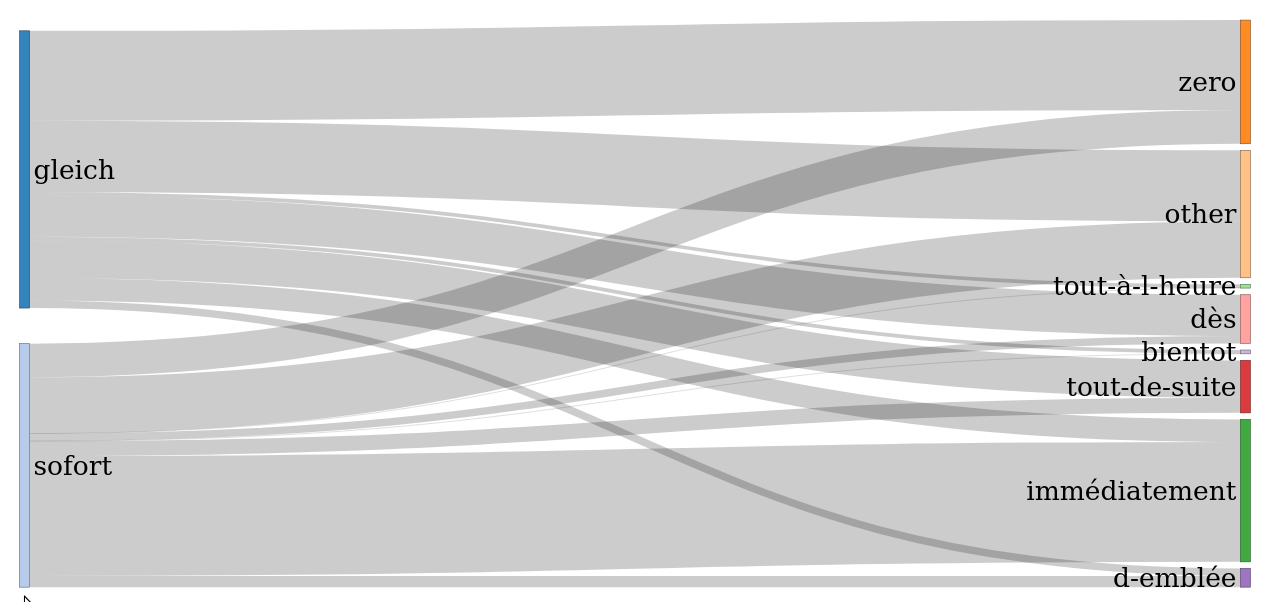
\includegraphics[width=0.85\linewidth]{figures/Sankey-de-fr.png}
  \cprotect\caption{Sankey plot showing French translations of the German
    \ipadv s \textit{gleich} and \textit{sofort}. The plot was
    generated with the package \verb+networkD3+ for \verb+R+
    \citep{networkD3-package}.}
  \label{fig:SankeyDeFr}
\end{figure}

We can add more information to `plain' Sankey diagrams by including an
intermediate layer of nodes displaying the frequencies of the levels of
some variable relative the source and target expressions, as in Figure
\ref{fig:SankeyDeFrRef}. The plot shows the frequencies of source and target
language correspondences mediated by the variable \textsc{Reference
point}. We can see that most cases of `deic[tic]-dir[ect]' come
from \textit{gleich} and go to `zero' or `other' (in French), while
almost all cases of `deic[tic]-phant[asma]' come from \textit{sofort}
and go to \textit{immédiatement}. Cases of `chron[ological]-ev[ent]'
seem to be typically associated with \textit{sofort} in German
originals, and with \textit{immédiatement} in French translations.

\begin{figure}[t]
  \centering
  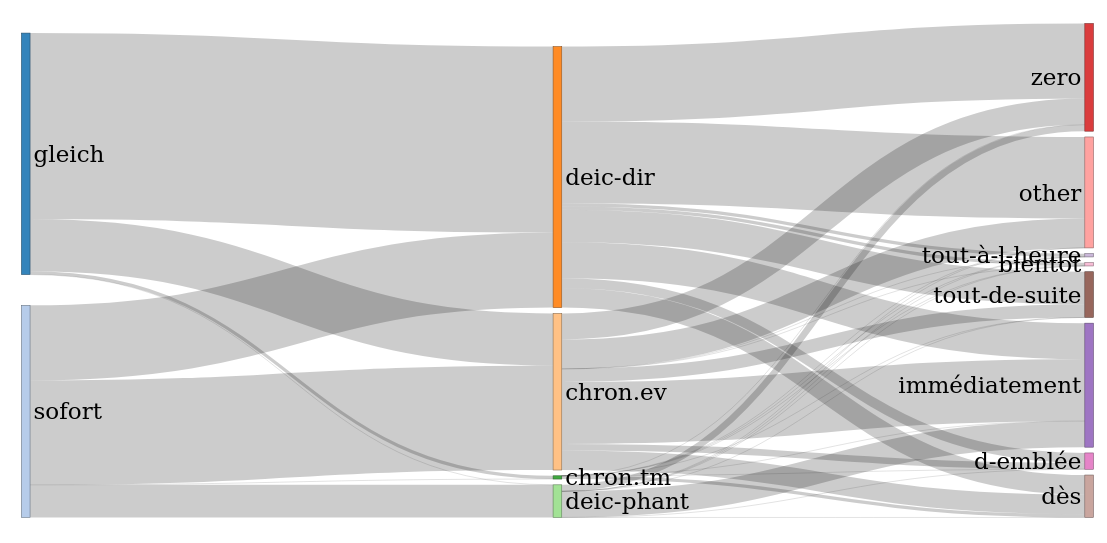
\includegraphics[width=0.9\linewidth]{figures/Sankey-de-fr-ref.png}
  \cprotect\caption{Comparative Sankey plot showing associations of
    IP-adverbials with French IP-adverbials, given the value for the
    variable \textsc{Reference point}. The plot was generated with the package
    \verb+networkD3+ for \verb+R+ \citep{networkD3-package}.}
  \label{fig:SankeyDeFrRef}
\end{figure}

To obtain a more global view, consider Figure
\ref{fig:SankeyDeFrCluster}, which shows the correspondences between
source and target language expressions relative to the clusters
mentioned in Sect. \ref{sec:ComparativeUndirected} (solution with
three clusters). We already know that Cluster 1 is positively associated
with \textit{gleich} in German. The plot shows that most cases of this
category go to `zero' or `other' in French. Clusters 2 and 3 are
more evenly distributed among \textit{gleich} and \textit{sofort} in
German, but they also seem to exhibit clear asymmetries.

While Sankey plots contain useful (relational) information about
frequency distributions in the source and target language, they do not
contain by-item information and are potentially deceptive. The edges
conecting the nodes reflect frequencies, but the left edges are not
connected by-item to the right edges. For example, as mentioned above,
if we look at the middle node `chron.ev' (for `chronological relative
to an event'), the plot suggests that those cases that are rendered
with \textit{gleich} in German go to `zero' and `other' in
French. While this is probably true, the underlying data does not
actually contain that information. Like a CA, Sankey diagrams are
built on cross-tables and merely represent frequencies of combinations
of levels for pairs of crossed variables. For example, it would be
conceivable that most or even all occurrences of \textit{sofort} going
to `deic-dir' actually end up at `zero'.

\begin{figure}[t]
  \centering
  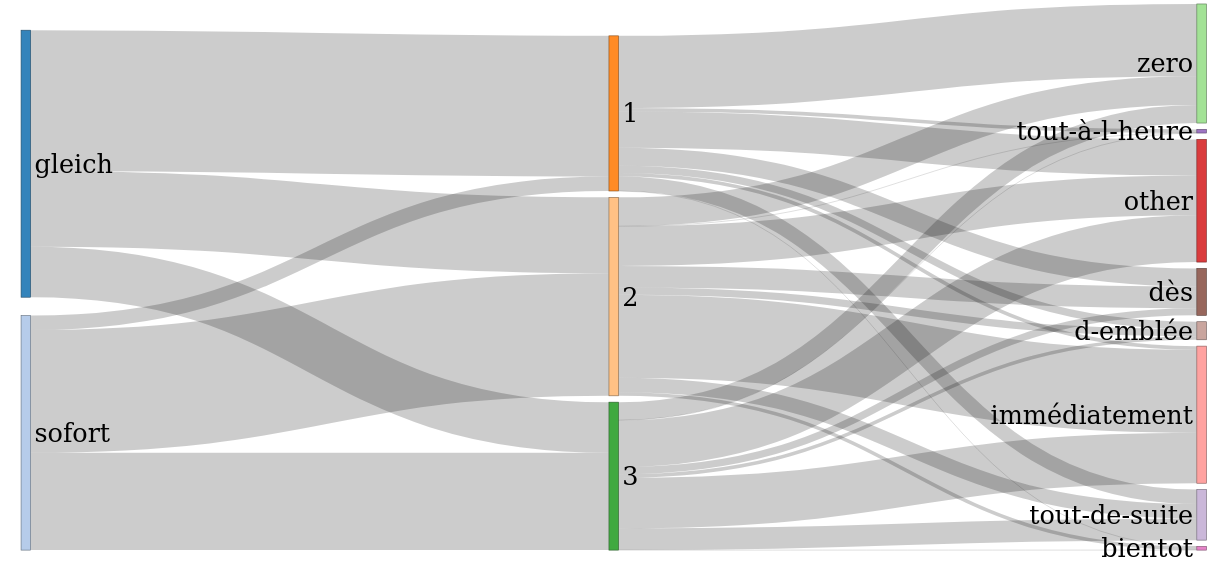
\includegraphics[width=0.9\linewidth]{figures/Sankey-de-fr-pam-low.png}
  \cprotect\caption{Comparative Sankey plot showing associations of
    IP-adverbials with French IP-adverbials, given a specific context
    cluster (solution with three clusters). The plot was generated with
    the package \verb+networkD3+ for \verb+R+
    \citep{networkD3-package}.}
  \label{fig:SankeyDeFrCluster}
\end{figure}


Translation choices can be represented more precisely with
visualizations that we call Context-Conditional Translation Graphs (CCTG; see also
\citealt{GastAtayan2019}). Consider the graph in Figure
\ref{fig:NetworkDeFr}.  It shows frequencies of choices made in
German-to-French translation, under specific contextual
conditions. The colours of the edges correspond to the three clusters
of context variables (see also the caption of the graph).
%
Figure \ref{fig:NetworkDeFr} shows that \textit{gleich} is indeed
mostly not translated at all in Context 1. \textit{Sofort} typically
goes to \textit{immédiatement} in Contexts 2 and 3. Unlike suggested
by Figure \ref{fig:SankeyDeFrCluster}, there does not seem to be any
particular association between \textit{gleich} and `other', as the
three arrows between these nodes have approximately the same width.

\begin{figure}[t]
  \centering
  % 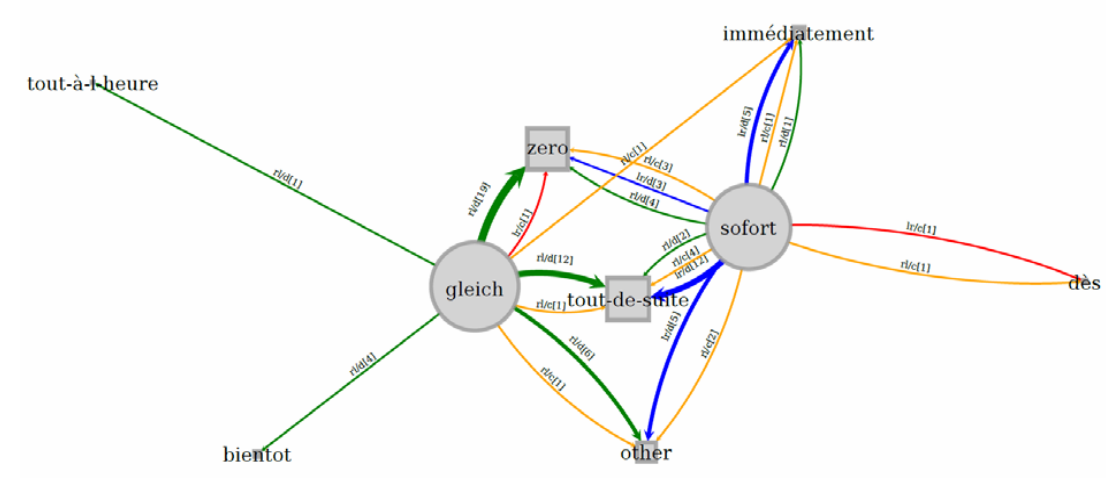
\includegraphics[width=\linewidth]{figures/TranslationGraphDeFr.png}
  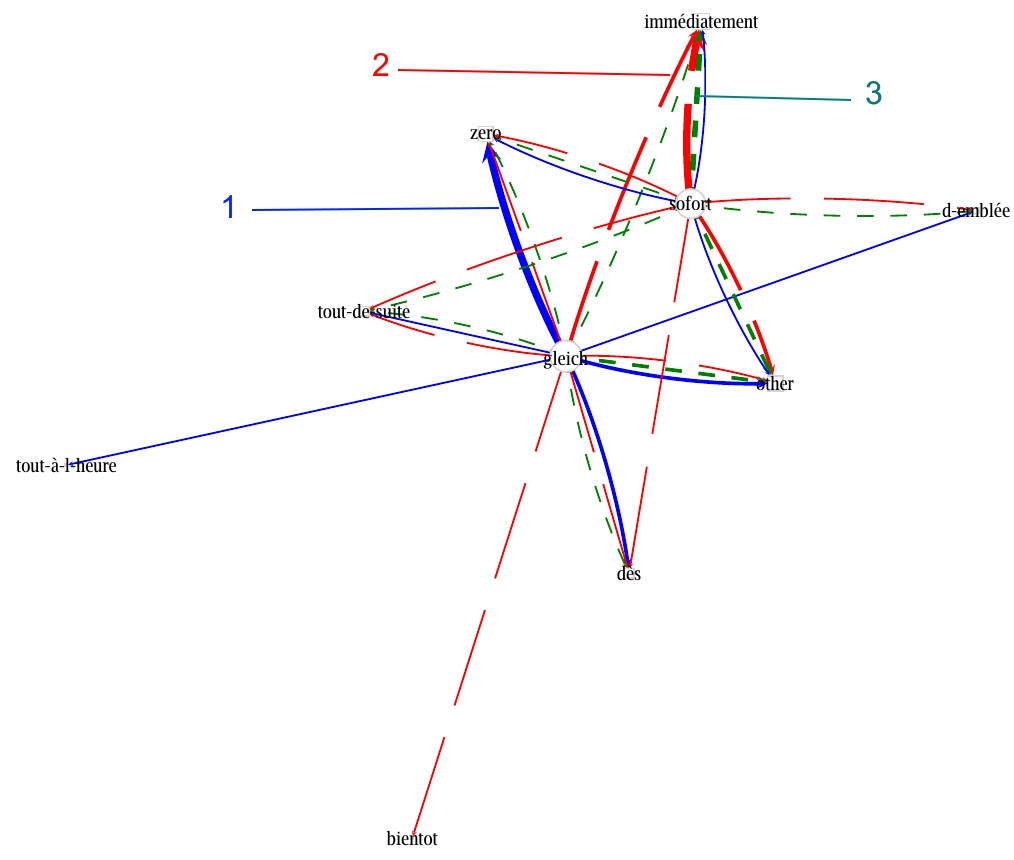
\includegraphics[width=\linewidth]{figures/network-de-fr.jpg}
  \cprotect\caption{Context-Conditional Translation Graph showing French
    translation choices for German \textit{gleich} and
    \textit{sofort}, given specific context clusters. The (solid) blue
    edge indicates translation in Context 1, the (long-dashed) red
    line represents translations in Context 2, and the (short-dashed)
    green line corresponds to Context 3. The graph was generated with
    the package \verb+graph_tool+ for \verb+Python+
    (https://graph-tool.skewed.de/static/doc/); see the script \verb+IpNetwork.py+ in the Supplementary Materials.}
  \label{fig:NetworkDeFr}
\end{figure}

%Once again, we wish to emphasize that impressions based on visualizations like the one in Figure \ref{fig:NetworkDeFr} should of course be supported by statistical evidence. 
%We will now sketch out ways of handling translation data using methods from Bayesian statistics.





%%% Local Variables:
%%% mode: latex
%%% TeX-master: "main"
%%% End:




\subsection{Bayesian networks}\label{sec:GraphicalModels}

In Section \ref{sec:Background} it was mentioned that choices in translation
can be regarded as coming with a specific conditional probability.
%
% One way of dealing with the inter-dependencies of observations in
% translated data is resorting to frameworks that make use of
% conditional probabilities.
For example, we can compare the conditional probability of finding
\textit{immédiatement} in Context 2 if there is
\textit{gleich} in the German original with its conditional
probability if there is \textit{sofort} in the original. That
would tell us something about the relationships between context types in
the original, expressions in the original and expressions in the
target language (note that translators may of course also choose to
change the context type, in which case we have to deal with yet
another variable determining the probabilities of using a specific
expression in the target language). While we cannot offer a complete
and statistically sound analysis of this type, we will present a
general framework which is flexible enough to accommodate such cases,
and that makes use of visualizations, more specifically, graphical models.

Graphical models capture the type of complex data structure as
encountered in translation studies in the form of networks or graphs
representing dependencies between random variables
(cf. \citealt{KollerFriedman2009}). We will use Bayesian networks, a
type of graphical model that represents the (assumed, hypothesized)
causal relations between variables. We will not be concerned with the
causal relationships between specific distributional variables. For
example, it seems reasonable to assume that \textsc{Illocutionary
  force} has a causal effect on the variables \textsc{Agent} and
\textsc{Intentionality}; if a speaker wants an addressee to do
something, that implies a certain amount of control on the part of the
addressee. This way of causal modeling is not specific to the type of
distribution under discussion in this section, i.e., choices made in a
target language under the influence of a source language expression.
 
It should be noted that corpus linguistic methods are not adequate for
investigating causal relationships in the process of bilingual
language production. We would need experimental evidence for
that. What we can do with corpus data, however, is model the cognitive
processes during translation and test the predictions derived from
this modeling. A simple example of a model of bilingual
language production is shown in Figure \ref{fig:BilingualModel} in the
form of a directed acyclic graph (DAG).\footnote{The graph was
  generated with the package \verb+bnlearn+ for \verb+R+. In Python,
  the module \verb+pgmpy+ can be used for Bayesian networks.} It represents the
choice of a French \ipadv\ in a translation from German. The nodes
represent variables, and they are associated with local probability
distributions:

\begin{figure}
  \centering
  %\begin{minipage}{5in}
 \begin{picture}(300,400)(0,100)
   \put(0,200){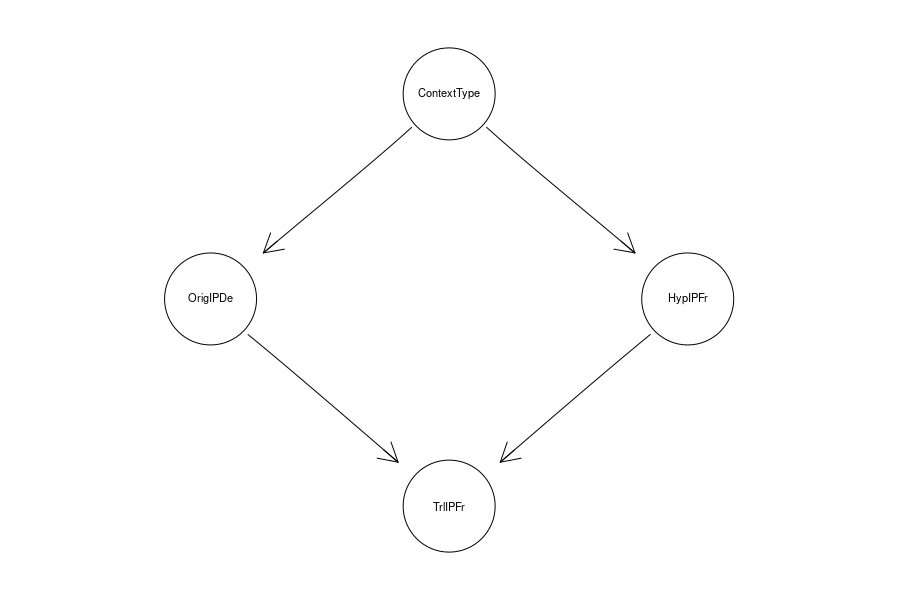
\includegraphics[width=0.9\linewidth]{figures/bilingual-model.jpeg}}
   \put(100,410){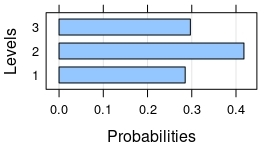
\includegraphics[width=0.3\linewidth]{figures/ProbsContextType.jpeg}}
   \put(0,340){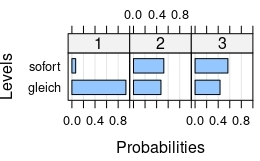
\includegraphics[width=0.3\linewidth]{figures/CondProbsOrigIPDe.jpeg}}
   \put(215,340){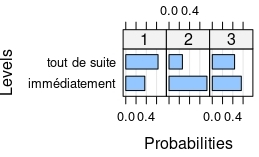
\includegraphics[width=0.3\linewidth]{figures/CondProbsHypIPFr.jpeg}}
   \put(30,110){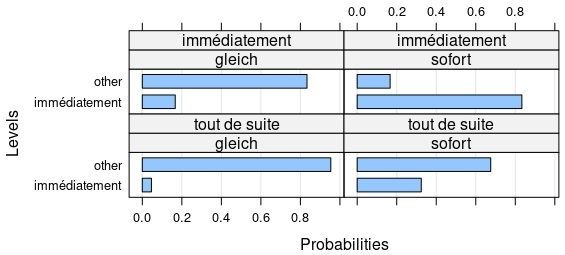
\includegraphics[width=0.6\linewidth]{figures/CondProbsTrlIPFr.jpeg}}
 \end{picture}
 %\end{minipage}
  \cprotect\caption{Directed acyclic graph for IP-adverbials
     (comparative/directional, with clustered observations). The graph
     was created with the package \verb+bnlearn+ for \verb+R+ \citep{bnlearn-package}.}
   \label{fig:BilingualModel}
\end{figure}


%\begin{itemize}
%\item
  The distribution of \textbf{Context types} is represented at the top of
  the graph. We assume the three types distinguished by the
  `smaller' PAM-cluster solution
  (cf. Sect. \ref{sec:ComparativeUndirected}). Each of the context
  types has a certain (relative) frequency. 
We estimated the frequencies of the three context types from our sample.

% \item
The specific context type conditions a frequency distribution in the
originals. We can, again, determine this distribution on the basis of
our sample. The node \textbf{OrigIPDe} is associated with conditional
probabilities of the form $p(w_{de}|c)$ -- the probability of using
a specific German \ipadv $w_{de}$, given a context $c$.

% \item
The node \textbf{HypIpFr} stands for a hypothetically used French \ipadv\ --
the \ipadv\ that \textit{may} have been used in monolingual (French) language
production, in the specific context. Like the node OrigIPDe, this
node is associated with a conditional frequency distribution,
$p(w_{fr}|c)$. This distribution can be estimated from the original
French data.

% \item
Finally, the node \textbf{TrlIPFr} stands for the \ipadv\ used in the French
translation from German. According to the DAG in Figure
\ref{fig:BilingualModel}, this choice is conditioned by the
probability of using a specific French expression (as in monolingual
language production), and the influence from the German \ipadv,
reflecting form-to-form associations in translation. 
The node TrlIPFr thus represents a distribution over French \ipadv s,
conditioned by the hypothetical French \ipadv\ and the German \ipadv\
in the original sentence. % In order to define this distribution, we
% infered the use of a French IP-adverbial based on the associations
% between context types and original French data.
This distribution cannot be observed, as no (hypothetical) monolingual
\ipadv\ is ever produced in French translation from German. In order
to infer the hypothetical French expressions, we trained a classifier
(a support vector machine/SVM) on all explanatory variables, predicting a
given \ipadv\ for each translated French sentence.\footnote{The
  model has an accuracy of 88.2\% for the entire training set, and of
  79.5\% with a 0.9/0.1 training/test split, averaging over ten-fold
  cross-validation. We used a radial kernel, with $C=3$ and
  $\gamma=0.1$.}
%\end{itemize}

The network shown in Figure \ref{fig:BilingualModel} represents a
hypothesis about mediated language production.  By breaking down the
joint probability distribution into local, partially independent
distributions, we can model components of the highly complex process
of mediated language production.
%
As our data set is quite small and the estimates for some parameters
are not very precise, we will illustrate this procedure with a binary
choice, by modeling the use of \textit{immédiatement} in French
translations. All French \ipadv s other than \textit{immédiatement}
were subsumed under the category of `other'.

The Bayesian network in Figure \ref{fig:BilingualModel} allows us to
determine theoretical distributions of French \ipadv s under
different conditions, and to compare them to the empirical
distributions. This can give us an estimate of the plausibility of the
causal model.
%
Tables \ref{tab:ProbTab} shows the empirical probabilities on the left
and the theoretical probabilities (according to the Bayesian network)
on the right. While the ranks of the expressions -- by context type
and \ipadv\ -- are identical, the two distributions are considerably
different. Even though the model in the form displayed in Figure
\ref{fig:BilingualModel} may not be entirely realistic, it provides
a starting point for a more elaborate model. This
is one of the main assets of Bayesian networks: they can be extended
and built up step by step, and their graphical nature helps
researchers to develop an understanding of the data.

\begin{table}[t]
  \begin{tabular}{l|ll|ll}
            & \multicolumn{2}{c|}{empirical} & \multicolumn{2}{c}{theoretical}\\\cline{2-5}    
ContextType &  \textit{gleich}     &   \textit{sofort}  & \textit{gleich} & \textit{sofort} \\\hline
1           & 0    & 0.25 & 0.09     & 0.51\\
2           & 0.24 & 0.53 & 0.13      & 0.7\\
3           & 0.07 & 0.48 & 0.11      & 0.61\\
  \end{tabular}
  \cprotect\caption{Empirical probabilities (left) and theoretical probabilities
    according to the Bayesian network (right) for the occurrence of
    \textit{immédiatement} in French translations, in specific
    contexts, given a specific German \ipadv\ in the original.}
  \label{tab:ProbTab}
\end{table}


%%% Local Variables:
%%% mode: latex
%%% TeX-master: "main"
%%% End:



\section{Conclusions and outlook}\label{sec:Conclusions}

The present chapter has provided an overview of various types of
methods used in comparative corpus linguistics and translation and
interpreting studies. Some of the methods are well known, -- e.g.,
mosaic plots (as in Figure \ref{fig:mosaicplots1-2}) -- while others
may be less familiar to parts of the community of contrastive
linguists and translation
scholars.

We discussed two major types of ordination: CA (with and without
stacking), and MCA (with and without supplementary variables). We made
an effort to convey an intuitive understanding of the mathematics
underlying these techniques. Users have to make specific choices and
decisions, e.g., CA vs. MCA, the type of map (symmetric, asymmetric,
row principal, etc.), and such decisions need to be
informed.
%
We also highlighted the connection between (M)CA and the familiar
Chi-squared statistic (e.g., the connections between this statistic
and Chi-squared distance, inertia, and the $\phi$-coefficient).

It seems to us that graph-based methods have some potential that has
not fully been exploited. Context-Conditional Correlation Graphs
(CCCGs, cf. Sect. Fig. \ref{fig:CCCG} in
Sect. \ref{sec:LanguageSpecific}) allow us to represent a large amount
of information about pairwise associations between variables in a
single plot. Sankey diagrams (Figures \ref{fig:SankeyDeFr},
\ref{fig:SankeyDeFrRef} and \ref{fig:SankeyDeFrCluster}), which are
commonly used in other fields, do not seem to be widespread in
translation studies, though they offer a very good way of summarizing
directional data. Translation graphs visualize choices made in
translation, under specific conditions. While the type of graph that
we provided (Figure \ref{fig:NetworkDeFr} in
Sect. \ref{sec:ComparativeDirected}) does not contain any type of
statistical information, such information could be added, potentially
using Bayesian statistical reasoning as outlined in
Sect. \ref{sec:GraphicalModels}, where we presented a type of
graphical model, i.e., Bayesian networks.

Once again, we would like to remind readers that the purpose of
the present chapter was not to present research results about \pradv
s. The data was mainly used for the purpose of illustration.  As
previously mentioned, more thorough studies on \pradv s were presented
in earlier publications of ours
\citep{Atayanetal2019,GastAtayan2019,Gastetal2019,Atayan2021b,Atayan2021a},
where some of the visualizations presented in this chapter were also
used.


%%% Local Variables:
%%% mode: latex
%%% TeX-master: "main"
%%% End:


\sloppy

\printbibliography[heading=subbibliography,notkeyword=this]


\begin{paperappendix}
\section{}

\subsection{Notes on Sect. \ref{sec:LanguageSpecific}}\label{sec:PearsonResds}

%\subsection{Pearson distribution and Pearson residuals}

When dealing with categorical data as discussed in this chapter, we
typically want to know if two or more variables correlate. In other
words, we want to know if a property of some observation -- a level of
a variable -- allows us to make inferences about some other property
of that observation.
%
According to the null hypothesis (of statistical independence), which
says that the two variables are unrelated, the conditional probability
of observing a specific property $A$ in some observation $x$, given
some other property $B$ of $x$, is identical to the probability of
observing $A$ in $x$ independently of $B$ (cf. \bv{condprob}). Put
differently, the probability of any $x$ exhibiting both $A$ and $B$ is
the product of the probabilities of $A$ and $B$ (cf. \bv{conjprob}).

\begin{exe}
  \ex\label{indep} Assumption of independence:
  \begin{xlist}
    \ex\label{condprob} $p(A|B)=p(A)$
    \ex\label{conjprob} $p(A\wedge B) = p(A)\cdot p(B)$
  \end{xlist}
\end{exe}
%
If two variables do not correlate, the frequencies in a
contigency table will be proportional along both dimensions.
Consider Table \ref{tab:contingencyschema}.
%

\begin{table}[h]
  \begin{tabular}[h]{l|ll|l}
          &  A: level 1 & A: level 2 & $\Sigma$\\\hline
    B: level 1   &  a & b & a+b\\
    B: level 2   &  c & d & c+d\\\hline
    $\Sigma$ & a+c & b+d & a+b+c+d\\
  \end{tabular}
  \caption{Schematic contingency table}
    \label{tab:contingencyschema}
\end{table}

If the variables $A$ and $B$ are independent of each other, we expect
the ratio of any two pairs of cells $\frac{c_1}{c_2}$ and
$\frac{c_3}{c_4}$ to be the same if $c_1$ and $c_2$, and $c_3$ and
$c_4$, are in the same column, and $c_1$ and $c_3$, and $c_2$ and
$c_4$, are in the same row (including the marginal row and column
sums). For instance:

\begin{exe}
  \ex
  \begin{xlist}
    \ex $\frac{a}{c}=\frac{b}{d}$
    \ex $\frac{a}{a+c}=\frac{b}{b+d}$
    \ex $\frac{a}{c}=\frac{a+b}{a+b+c+d}$
    \ex $\frac{a}{b}=\frac{c}{d}$
    \ex $\frac{a}{a+b}=\frac{c}{c+d}$
    \ex\label{abcd} $\frac{a}{a+c}=\frac{a+b}{a+b+c+d}$
  \end{xlist}
\end{exe}
%
Based on such analogies, we expect the following count for cell $a$,
under the assumption of statistical independence of the variables. The
equation in \bv{ahat} follows from \bv{abcd} by multiplication with
$(a+c)$ (the symbol $\hat{\phantom{a}}$ on the $\hat{a}$ indicates that this variable
represents an expected value).

\begin{exe}
      \ex\label{ahat} $\hat{a}=\frac{(a+c)(a+b)}{a+b+c+d}$   
\end{exe}
%
The difference between the observed frequency $a$ and the expected
frequency $\hat{a}$ provides a way of determining
deviations from statistical independence.

In what follows we use the matrix formalism, which provides a compact
way of expressing and generalising the above example. $C$ represents
the original contingency table, and $\hat{C}$ corresponds to the
matrix of the expected frequencies as calculated from the independence
condition as stated in \ref{indep}.
%
The matrix of \textbf{Pearson residuals} is then calculated as:

\begin{exe}
  \ex Pearson residuals\\$R=(C-\hat{C})/\sqrt{\hat{C}}$
\end{exe}
%
The matrix
$\sqrt{\hat{C}}$ contains the square roots of the cells in
$\hat{C}$. Division by the square root of the expected value is a
standardization step. We assume Poisson sampling (independent
selection of subjects), so each cell is assumed to follow a Poisson
distribution. In a Poisson distribution, the variance is equal to the
expected value (both values are represented by the parameter
$\lambda$). We divide the difference between the expected and the
observed value by the square root of the variance -- the standard
deviation -- to standardize the values.

In matrix notation, the matrix of expected values $\hat{C}$ can be
represented as follows:

\begin{exe}
  \ex\label{PearsonDef}
  \begin{xlist}
    %\ex $R=(C-\hat{C})/\sqrt{\hat{C}}$,
    \ex $\hat{C}=(m_m\otimes m_n)/N$, (the outer product of row and
    column margins, divided by the number of
    observations) %$\sum_{0=1}^m\sum_{0=1}^nC_{m,n}\times m_m\otimes
                  %m_n$,
    \ex   $m_m=1C, m_n=1C^\mathsf{T}$, (row and column sums)
    \ex   $N=1^\mathsf{T} C1$ (the sum of all cells)
  \end{xlist}
  %$m_m$ and $m_n$ being the row and column masses, respectively.  
\end{exe}
%
The \textbf{adjusted Pearson residuals} are obtained 
as shown in \bv{adjresid}. We divide the difference between the
observed and the expected value by an estimate of the standard error
based on the assumption that the marginal sums are fixed, therefore
assuming a hypergeomteric distribution. Adjusted Pearson residuals are
always larger than unadjusted Pearson residuals, as the additional
term in the demoninator -- $\sqrt{(1-m_m/N)(1-m_n/N)}$ -- is always
smaller than 1.

\begin{exe}
  \ex\label{adjresid} $\tilde{r}=\frac{C-\hat{C}}{\sqrt{\hat{C}(1-m_m/N)(1-m_n/N)}}$
\end{exe}

\subsection{Notes on ordination}\label{sec:AppOrdination}

The information in this section is mainly intended to facilitate an
intuitive understanding of the methods. For more complete and more
accurate information, please consult \citet{Greenacre2016}.

\subsubsection*{Some terms and concepts}

A \textbf{contingency table} is a table with counts of observations
with specific properties, cf. Table \ref{tab:contingency}.

\begin{table}[ht]
\centering
\begin{tabular}{r|rrr|r}
  \hline
 & comm & dir.boul & repr & $\Sigma$\\ 
  \hline
  \textit{gleich}       &   4 &   3 &  18 & 25      \\ 
  \textit{sofort}       &   2 &  14 &  18 & 34\\ 
  \textit{unverzüglich} &   1 &   6 &   2 & 9 \\\hline
  $\Sigma$       &   7 &  23 &  38 & 68 \\
   \hline
\end{tabular}
\caption{Contingency table}
\label{tab:contingency}
\end{table}

A \textbf{percentage table} shows the relative frequency of each cell,
i.e., the cell value divided by the number of observations (cf. Table
\ref{tab:percentage}).  The \textbf{row} and \textbf{column masses}
(the margins of Table \ref{tab:percentage}) are the relative
frequencies of all observations in specific rows or columns.

\begin{table}[hb]
\centering
\begin{tabular}{r|rrr|r}
  \hline
 & comm & dir.boul & repr & $\Sigma$\\ 
  \hline
  \textit{gleich} & 0.06 & 0.04 & 0.26 & \textbf{0.37}\\ 
  \textit{sofort} & 0.03 & 0.21 & 0.26 & \textbf{0.50}\\ 
  \textit{unverzüglich} & 0.01 & 0.09 & 0.03 & \textbf{0.13}\\ 
  \hline
  $\Sigma$               & \textbf{0.11}   & \textbf{0.34}    &  \textbf{0.56}   &    1\\
\end{tabular}
\caption{Percentage table}
\label{tab:percentage}
\end{table}

The \textbf{profile} of a given category constituting the row of a
contingency or percentage table is the rowwise proportion of that
category (cf. Table \ref{tab:profile}).

\begin{table}[ht]
\centering
\begin{tabular}{r|rrr|r}
  \hline
 & comm & dir.boul & repr & $\Sigma$\\ \hline
  \textit{gleich} & 0.16 & 0.12 & 0.72 & 1\\ 
  \textit{sofort} & 0.06 & 0.41 & 0.53 & 1\\ 
  \textit{unverzüglich} & 0.11 & 0.67 & 0.22 & 1\\ \hline
\end{tabular}
\caption{Row profiles}
\label{tab:profile}
\end{table}

The \textbf{average profile} -- geometrically speaking the
\textbf{centroid} -- is the average of the row profiles, weighted by
the row masses. For the first column:

 \begin{exe}
   \ex $\hat{c_1} = 0.37 \cdot 0.16 + 0.5 \cdot 0.06 + 0.13 \cdot 0.11 = 0.1$
 \end{exe}
%
 The average profile for Table \ref{tab:contingency} is thus:

 \begin{exe}
   \ex $\hat{C}_{j+} = (0.1\; 0.34\; 0.56)$
 \end{exe}
%
 We can obtain a \textbf{standardized profile table} by scaling the columns of
 the profile table (Table \ref{tab:profile}) by the inverse of the
 square root of the average profile values (i.e., we divide each value
 by the square root of the corresponding average profile value).
 For example, the average profile value of the first column is $0.1$,
 and its square root is $\approx 0.32$. If we divide $0.16$ (the first
 value of the profile of \textit{gleich}) by $0.32$, we obtain a value of
 $0.5$:

\begin{table}[ht]
\centering
\begin{tabular}{rrrr}
  \hline
 & 1 & 2 & 3 \\ 
  \hline
  gleich & 0.5 & 0.21 & 0.96 \\ 
  sofort & 0.18 & 0.71 & 0.71 \\ 
  unverzüglich & 0.35 & 1.15 & 0.30 \\ 
   \hline
\end{tabular}
\caption{Standardized profile table}
\end{table}
%
In a coordinate system scaled by the inverse of the square root of the expected
value Euclidean distances are equivalent with Chi-squared distances.

The \textbf{Chi-squared distance} $\chi^2_{\Delta}$ is the square root
of the sum of the squared differences between the observed values and
the expected values, divided by the expected values.
%
For each row $m$ of a matrix $C_{m\times n}$:
\begin{exe}
  \ex
  $\chi^2_{\Delta,m} =
  \sqrt{\sum_{i=1}^{n}{\frac{(C_{m,i}-\hat{C}_{m,i})^2}{\hat{C}_{m,i}}}}$

  ($\hat{C}$ being the matrix of expected values, see (\ref{PearsonDef}))

\end{exe}
%
The sum of the Chi-squared distances of a matrix provides the basis
for the concept of \textbf{inertia} in Correspondence Analysis. The
inertia of a contingency table is %the weighted average of the
% Chi-square distances of each row to the row profile, where the average
% is weighted by the row masses $M$
``the weighted average of the squared $\chi^2$ -distances between the
row profiles and their average profile'' \citep[29]{Greenacre2016}. It is 
weighted by the row masses $M$.
For a matrix  $C_{m\times n}$,

\begin{exe}
  \ex $I_C=\sum_{i=1}^m\sum_{j=1}^nM_i\frac{(C_{i,j}-\hat{C}_{i,j})^2}{\hat{C}_{i,j}}$.
\end{exe}
%
Note that the Chi-squared distance is identical to the Chi-squared
value of a table, divided by the number of observations, and that it
is equivalent to the $\phi$-coefficient squared, so
$\phi=\sqrt{\chi^2/n}$.

\subsubsection*{Singular value decomposition}\label{sec:SVD}

As a starting point of singular value decomposition,
we use a table of standardized residuals. It is
obtained just as was in described in Sect. \ref{sec:PearsonResds} for the
Pearson residuals. However, in Correspondence Analysis we calculate
standardized residuals from a percentage table as shown in Table
\ref{tab:percentage}, not from a contingency table as shown in Table
\ref{tab:contingency}. The two tables differ by a factor of
$\sqrt{N}$, i.e., in our case, $8.246$ (=$\sqrt{68}$). Table
\ref{tab:StandResds} contains standardized residuals.

\begin{table}[ht]
\centering
\begin{tabular}{rrrr}
  \hline
                        & comm & dir.boul & repr \\ 
   \hline
  \textit{gleich}       & 0.11 & -0.23 & 0.13 \\ 
  \textit{sofort}       & -0.10 & 0.09 & -0.03 \\ 
  \textit{unverzüglich} & 0.01 & 0.21 & -0.16 \\ 
   \hline
\end{tabular}
\caption{Table of standardized residuals}
\label{tab:StandResds}
\end{table}



\begin{figure}[t]
  \centering
  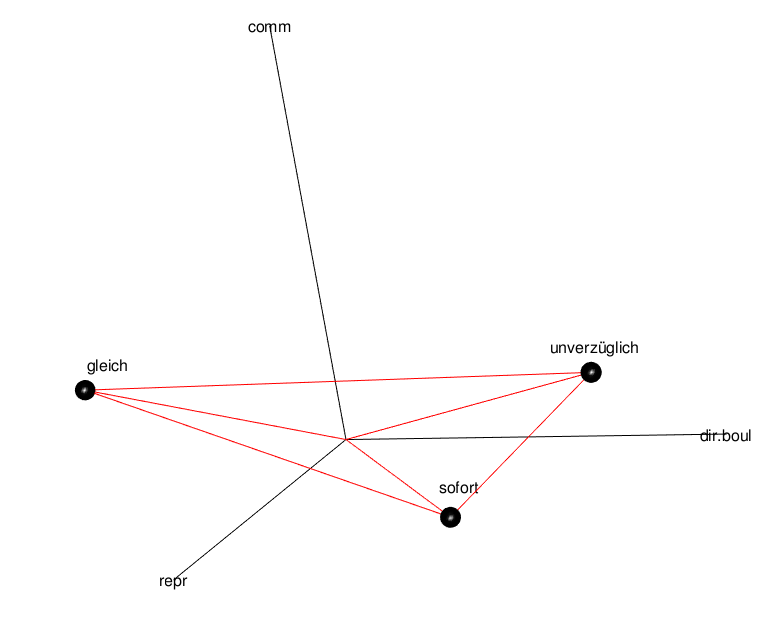
\includegraphics[width=0.5\linewidth]{figures/Ordination3b.png}
  \caption{Visualizing the standardized residuals of Table \ref{tab:PropTable}}
  \label{fig:Ordination3App}
\end{figure}

We can represent Table \ref{tab:StandResds} in a three-dimensional
coordinate system as shown in Figure \ref{fig:Ordination3} in the main
text, which is repeated for convenience in Figure
\ref{fig:Ordination3App}.
%
Alternatively, we can think of Table \ref{tab:StandResds} as a mapping
from one three-dimensional coordinate system to another three-dimensional
coordinate system. Let us assume a source system that consists of three unit
vectors only, i.e., a standard basis (cf. Figure
\ref{fig:Ordination3App}). When regarded as a transformation map,
Table \ref{tab:StandResds} (via matrix multiplication) maps the
standard basis to the residuals shown in red in Figure \ref{fig:Ordination4App}. What matters here is
that by regarding the matrix as a transformation map we can not only
map the three standard vectors to new coordinates, we can map
\textit{any} point in the source system to the target system. For example,
the point located at $(0.5\; 0\; 0)$, which is halfway between the
origin and the unit vector $(1\; 0\; 0)$ in the original system, will be
mapped to a point that is halfway between the origin and the target
vector of $(1\; 0\; 0)$ in the new system (see the two orange points
in Figure \ref{fig:Ordination4App}).

\begin{figure}[t]
  \centering
  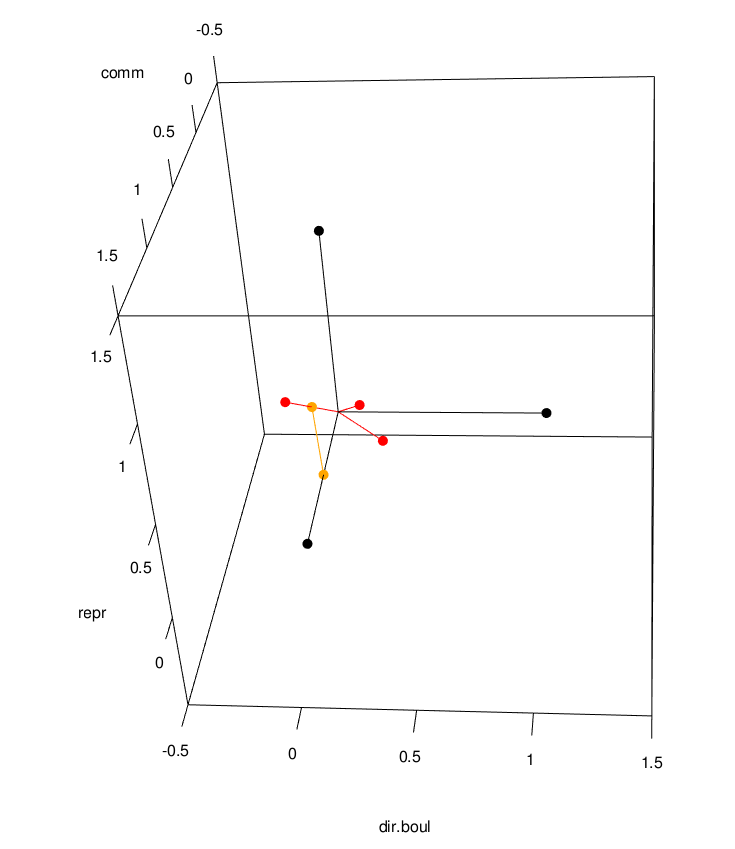
\includegraphics[width=0.5\linewidth]{figures/SVD3.png}
  \caption{Table \ref{tab:StandResds} as a mapping from a standard basis to a new coordinate system}
  \label{fig:Ordination4App}
\end{figure}

Under the transformation view of the matrix in Table
\ref{tab:StandResds} we can perform a `global' transformation of the
original coordinate system. Consider Figure \ref{fig:Sphere}, which shows a random
sample of vectors (represented as points) of unit length.  The cloud
of points shown in Figure \ref{fig:Sphere} can be mapped to the space
of standardized residuals in the same way in which we mapped the three
unit vectors to that space in Figure \ref{fig:Ordination3App} with
matrix multiplication. All points will be mapped to a `disc' that
contains the origin, see Figure \ref{fig:Ellipse}.

\begin{figure}[t]
  \centering
  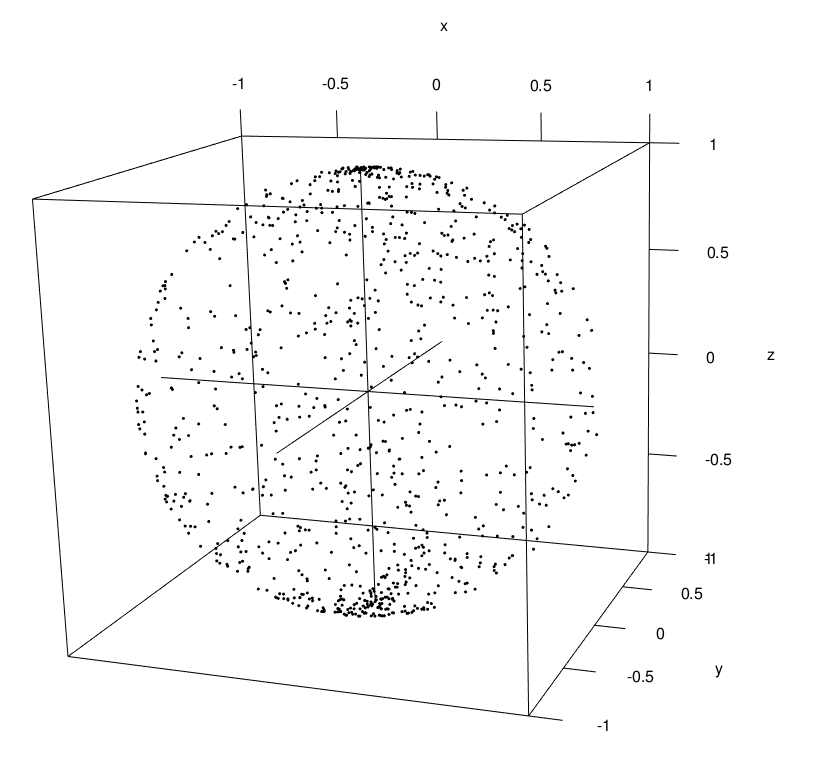
\includegraphics[width=0.5\linewidth]{figures/SVD4.png}
  \caption{A random sample of 1,000 vectors of length 1}
  \label{fig:Sphere}
\end{figure}


\begin{figure}[b]
  \centering
  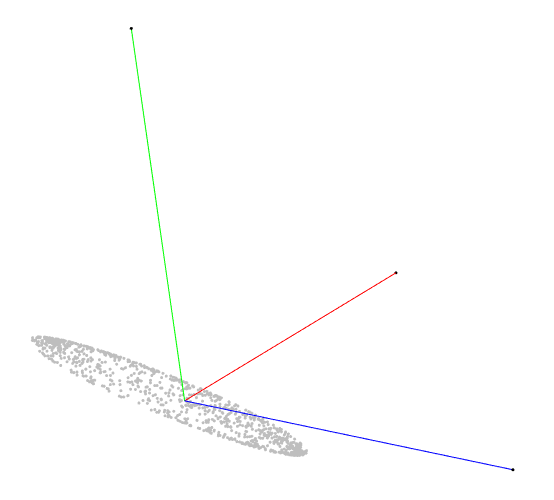
\includegraphics[width=0.5\linewidth]{figures/SVD5.png}
  \caption{The random sample of 1,000 vectors from Figure
    \ref{fig:Sphere} mapped to residual space}
  \label{fig:Ellipse}
\end{figure}

\pagebreak

We can now look at the `disc' of Figure \ref{fig:Ellipse} from a
different point of view, see Figure \ref{fig:Ellipse2}. This plot
shows two straight lines. The horizontal line points in the
direction in which the points of the new cloud are spread out most. It
is the first \textbf{singular vector}. The vertical line is orthogonal to the
horizontal line. It shows the direction in which the data is spread
out most, on the condition of being orthogonal to the first
line. (Note that there appears to be only one line that is orthogonal
to the first line, but remember that the disc is actually located in
three-dimensional space [see Figure \ref{fig:Ellipse}], so there are in
fact an infinite number of vectors that are orthogonal to the first
singular vector, pointing away from the disc).

\begin{figure}[t]
  \centering
  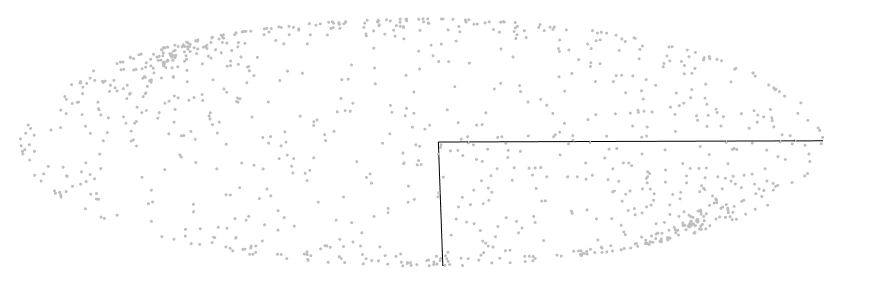
\includegraphics[width=0.5\linewidth]{figures/SVD6.png}
  \caption{The random sample of 1,000 vectors from Figure
    \ref{fig:Sphere} mapped to residual space, from a different perspective and with singular vectors}
  \label{fig:Ellipse2}
\end{figure}

Singular value decomposition is a method to find singular vectors and their lengths, the singular values.
It decomposes a matrix $M$ into two
square matrices $U$ and $V$ and a (rectangular diagonal) scaling matrix $\Sigma$ such
that:

\begin{exe}
  \ex\label{SVDFormula}  $M = U\Sigma V^*$
\end{exe}
%
where $^*$ denotes the conjugate transpose of a matrix. For matrices
of the type dealt with in the present context, the conjugate transpose
is identical to the transpose, i.e., $V^*=V^\mathsf{T}$.

The matrices $U$ and $V$ contain orthonormal bases as row and column vectors,
which means that these vectors are orthogonal to each other, and each vector is
of unit length. In the case of $U$, the row vectors are orthogonal, in
the case of $V$, it is the column vectors that are orthogonal, hence:

\begin{exe}
  \ex  $UU^T=I$
  \ex $V^TV=I$
\end{exe}
%
In our case, the SVD delivers the following
factorization (obtained with the function \verb+svd+ in R):

\begin{exe}
  \ex $U$ \hspace{3.7cm} $\Sigma$ \hspace{3.1cm} $V$
%\end{exe}

$\begin{bmatrix}
  -0.72 & 0.35 & 0.61 \\ 
   0.28 & -0.65 & 0.71 \\ 
   0.64 & 0.68 & 0.36 \\
\end{bmatrix}$
%
\hspace{1em}
  $\begin{bmatrix}
   0.39 & 0.00 & 0.00 \\ 
   0.00 & 0.12 & 0.00 \\ 
   0.00 & 0.00 & 0.00 \\ 
 \end{bmatrix}$
%
\hspace{1em}
%
  $\begin{bmatrix}
   -0.25 & 0.91 & -0.32 \\ 
   0.81 & 0.02 & -0.58 \\ 
    -0.52 & -0.41 & -0.75 \\
    \end{bmatrix}$
 \end{exe}
%
 To see that the first two row vectors of U are orthogonal (they stand in a $90^o$ angle to each other), consider their
 dot product:

 \begin{exe}
   \ex $u_1\cdot u_2$ \\
   $=(-0.715 \cdot 0.285) + (0.348 \cdot -0.647) + (0.606 \cdot 0.707)$\\
   $=-0.204 -0.225 + 0.429 = 0$
 \end{exe}
%
 To see that the length of the first vector is 1:

 \begin{exe}
   \ex $\sqrt{-0.715^2 + 0.348^2 + 0.606^2}$\\
   $=\sqrt{0.511 + 0.121 + 0.367}$\\
   $=\sqrt{1} = 1$
 \end{exe}
%
 The rows of $U$, and the columns of $V$, constitute the bases for the coordinates of the rows and columns in CA.
 %
 Both matrices are scaled by the inverse of the square root of the average profile values ($W_m, W_n$ below).
 %
 The matrix of interest is moreover scaled by the singular values in matrix $\Sigma$.
 %
 If we want to locate rows in a coordinated system defined by their associations with columns, we
 will only scale the left singular values, i.e., matrix $U$, by $\Sigma$.
 %
 If we want to locate columns in a coordinate system defined by their associations with rows, we scale the right singular values, i.e., matrix
 $V$, by $\Sigma$. Sets of coordinates, here represented as $C$, can thus be
 obtained as follows (in the text we were only interested in the row
 analysis):
 
 \begin{exe}
   \ex row analysis
   \begin{xlist}
   \ex $C_{row}= W_m U \Sigma$
   \ex $C_{col} = W_n V$     
   \end{xlist}
   \ex column analysis
     \begin{xlist}
   \ex $C_{col}= W_n V \Sigma$
   \ex $C_{row} = W_m U$     
   \end{xlist}
 \end{exe}
%
In an asymmetric map, where rows are represented in principal
coordinates and columns in standard coordinates, we can reconstruct
the original matrix from the map via the inner product between row and column
vectors. For example, the \ipadv\ \textit{gleich} and the column
`repr' have the following coordinates:

\begin{exe}
  \ex \textit{gleich}: $(-0.46\; 0.07)$
  \ex `repr': $(-0.70 -\!0.54)$ 
\end{exe}
%
These coordinates first need to be scaled by the square root of the row masses/average profile (to `undo' the scaling that was applied previously):

\begin{exe}
  \ex \textit{gleich}: $0.606\; (-0.463\; 0.067) = (-0.281\; 0.041)$
  \ex `repr': $0.748\; (-\!0.702\; -\!0.545) = (-\!0.525\; -\!0.407)$
\end{exe}
%
The inner product of these vectors is:

\begin{exe}
  \ex $-0.281\cdot -\!0.525 + 0.041\cdot -\!0.407=0.131$
\end{exe}
%
The result, $0.131$, is the standardized residual of the cell for \textit{gleich} and `repr'. 

\subsection{Notes on Sect. \ref{sec:ComparativeUndirected}}\label{sec:AppComparativeUndirected}

Figure \ref{fig:Silhouette} shows the silhouette plot for the
clustering reported on in Sect.  \ref{sec:ComparativeUndirected}.

\begin{figure}[h]
  \centering
  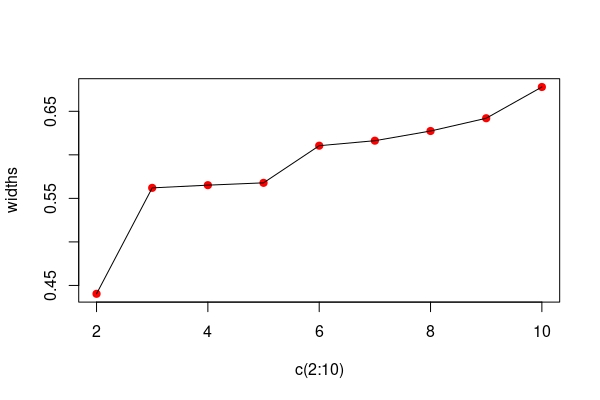
\includegraphics[width=0.5\linewidth]{figures/silhouette.jpeg}
  \caption{Silhouette widths for cluster solutions}
  \label{fig:Silhouette}
\end{figure}


%\subsection{Notes on Sect. \ref{sec:GraphicalModels}}\label{sec:AppGraphicalModels}



%\section{Notes on the chi-squared test}


%\section{Notes on ordination}







%%% Local Variables:
%%% mode: latex
%%% TeX-master: "main"
%%% End:
\end{paperappendix}



\end{document}
